%\documentclass[notes, c, 11pt, xcolor=dvipsnames, hyperref={colorlinks,citecolor=Maroon,linkcolor=Maroon,urlcolor=RoyalBlue}]{beamer}

% print notes only:
%\documentclass[notes=only, c, 11pt, xcolor=dvipsnames, hyperref={colorlinks,citecolor=Maroon,linkcolor=Maroon,urlcolor=RoyalBlue}]{beamer}

%print only frames:
\documentclass[c, 11pt, xcolor=dvipsnames, hyperref={colorlinks,citecolor=Maroon,linkcolor=Maroon,urlcolor=RoyalBlue}]{beamer}

% print handouts:
%\documentclass[handout, c, 11pt, xcolor=svgnames, hyperref={colorlinks,citecolor=DeepPink4,linkcolor=DarkRed,urlcolor=DarkBlue}]{beamer} 
%\usepackage{pgfpages}
%\pgfpagesuselayout{4 on 1}[a4paper, border shrink=5mm, landscape]

\setbeamerfont{note page}{size=\tiny}

\usepackage[english]{babel}
\usepackage[latin1]{inputenc}
\usepackage[T1]{fontenc}

\mode<presentation> {
	
	% The Beamer class comes with a number of default slide themes
	% which change the colors and layouts of slides. Below this is a list
	% of all the themes, uncomment each in turn to see what they look like.
	
	%\usetheme{default}
	%\usetheme{AnnArbor}
	%\usetheme{Antibes}
	%\usetheme{Bergen}
	%\usetheme{Berkeley}
	%\usetheme{Berlin}
	%\usetheme{Boadilla}
	\usetheme{CambridgeUS}
	%\usetheme{Copenhagen}
	%\usetheme{Darmstadt}
	%\usetheme{Dresden}
	%\usetheme{Frankfurt}
	%\usetheme{Goettingen}
	%\usetheme{Hannover}
	%\usetheme{Ilmenau}
	%\usetheme{JuanLesPins}
	%\usetheme{Luebeck}
	%\usetheme{Madrid}
	%\usetheme{Malmoe}
	%\usetheme{Marburg}
	%\usetheme{Montpellier}
	%\usetheme{PaloAlto}
	%\usetheme{Pittsburgh}
	%\usetheme{Rochester}
	%\usetheme{Singapore}
	%\usetheme{Szeged}
	%\usetheme{Warsaw}
	
	% As well as themes, the Beamer class has a number of color themes
	% for any slide theme. Uncomment each of these in turn to see how it
	% changes the colors of your current slide theme.
	
	%\usecolortheme{albatross}
	%\usecolortheme{beaver}
	%\usecolortheme{beetle}
	%\usecolortheme{crane}
	%\usecolortheme{dolphin}
	%\usecolortheme{dove}
	%\usecolortheme{fly}
	%\usecolortheme{lily}
	%\usecolortheme{orchid}
	%\usecolortheme{rose}
	%\usecolortheme{seagull}
	%\usecolortheme{seahorse}
	%\usecolortheme{whale}
	%\usecolortheme{wolverine}
	
	\usefonttheme{professionalfonts}
	
	\usepackage{times}
	\usepackage{tikz}
	\usetikzlibrary{arrows,shapes}
	
	%\setbeamertemplate{footline} % To remove the footer line in all slides uncomment this line
	%\setbeamertemplate{footline}[page number] % To replace the footer line in all slides with a simple slide count uncomment this line
	\setbeamertemplate{headline} % to remove header with navigation tree
	
	\setbeamertemplate{navigation symbols}{} % To remove the navigation symbols from the bottom of all slides uncomment this line
}

\usepackage{amsmath,mathtools}
\usetikzlibrary{matrix, fit, backgrounds}

\usepackage{graphicx} % Allows including images
\usepackage{booktabs} % Allows the use of \toprule, \midrule and \bottomrule in tables
\usepackage{subcaption}
\usepackage{tabularx}

\usepackage{fancyvrb}

\usetikzlibrary{mindmap,trees,shadows,backgrounds}

%\tikzset{every node/.append style={scale=0.6}}    

\usepackage{array,multirow}
\usepackage{changepage}

\usepackage[backend=biber, style=authoryear-comp, citestyle=authoryear-comp, firstinits=true, url=false, doi=false, eprint=false, dashed=false, maxbibnames=99]{biblatex}
\addbibresource{bib.bib}

%----------------------------------------------------------------------------------------
%	TITLE PAGE
%----------------------------------------------------------------------------------------

\title[Webinar for ISDS R Group]{Building meaningful machine learning models for disease prediction} % The short title appears at the bottom of every slide, the full title is only on the title page

\author{Dr Shirin Glander} % Your name
\institute[] % Your institution as it will appear on the bottom of every slide, may be shorthand to save space
{
	Dep. of Genetic Epidemiology \\
	Institute of Human Genetics \\
	University of M\"unster
	
	\vspace{0.5cm} 
	
	\href{mailto:shirin.glander@wwu.de}{shirin.glander@wwu.de} \\
	
	\vspace{0.5cm} 
	
	\href{https://shiring.github.io}{https://shiring.github.io} \\
	
	\href{https://github.com/ShirinG}{https://github.com/ShirinG}
	
}
\date{Friday, 31\textsuperscript{st} March 2017} 

\AtBeginSection[]{
	\begin{frame}
		\vfill
		\centering
		\begin{beamercolorbox}[sep=8pt,center,shadow=true,rounded=true]{title}
			\usebeamerfont{title}\insertsectionhead\par%
		\end{beamercolorbox}
		\vfill
	\end{frame}
}

%\renewcommand{\thefootnote}{$\star$} 

%%%%%%%%%%%%%%%%%%%%%
%	TITLE PAGE
%%%%%%%%%%%%%%%%%%%%%

\begin{document}

	\begin{frame}
		\titlepage
	\end{frame}
	
\note{
	\begin{itemize}
		\item Welcome everybody!
		\item Thank you very much for the invitation!
		\item In this presentation, I will go over my work on using machine learning models in disease prediction
		\item I want to specifically give a hands-on demonstration of how you can build meaningful models using R
		\item I will demonstrate how to evaluate model performance and
		\item how to optimize models to address different disease-related questions using a case study
		\item all slides and the complete code behind the figures produced in this presentation will be available to you after this talk
	\end{itemize}
}

%%%%%%%%%%%%%%%%%%%%%
%	ABOUT ME
%%%%%%%%%%%%%%%%%%%%%

\begin{frame}
	\frametitle{About me}
	
	\begin{columns}
		\column{0.15\textwidth}	
	
		\column{0.8\textwidth}	
	\begin{itemize}		
		\item[since 2015] Bioinformatics Postdoc \\
							Next Generation Sequencing \\
							autoinflammatory diseases \& \\
							innate immunity \\[5mm]
		\item[2011 - 2015] PhD in Biology \\
							Is the immune system of plants required to adapt to flowering time change? \\[5mm]
		\item[2005 - 2011] BSc and MSc of Science in Biology \\
							evolutionary genetics, \\ immune memory in Drosophila \\				
	\end{itemize}

	\column{0.05\textwidth}	
	
	\begin{tikzpicture}[remember picture,overlay]
	\node[xshift=-2.1cm,yshift=-2.5cm] at (current page.north east) {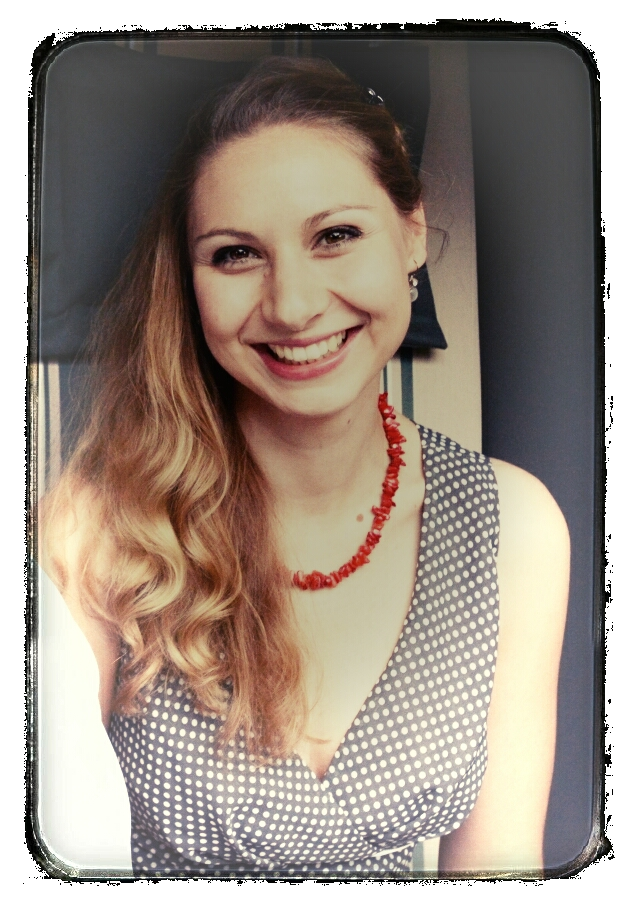
\includegraphics[width=3cm]{images/bild.png}};
	\end{tikzpicture}

	\end{columns}
\end{frame}

\note{
	\begin{itemize}
		\item Before I start, I want to quickly introduce myself:
		\item I am a bioinformatics postdoc
		\item working with next generation sequencing data,
		\item like RNA-seq for transcriptomics,
		\item whole genome sequencing for variant analysis,
		\item ATAC- or Chip-seq for chromatin and epigenetic information.
		\item My own research focuses on questions relating to autoinflammatory diseases
		\item and innate immune mechanisms
	\end{itemize}
	
	\begin{itemize}
		\item I earned my PhD in biology from the University of M�nster in 2015
		\item working with RNA-seq data to determine how plant defense has co-evolved with and potentially shaped different life-history strategies
	\end{itemize}
	
	\begin{itemize}
		\item Before that, during my BSc and MSc I worked on evolutionary genetics and immune memory in Drosophila
	\end{itemize}
	
	\begin{itemize}
		\item I am also an R-blogger and dance teacher in my spare time
	\end{itemize}
}

%%%%%%%%%%%%%%%%%%%%%
%	TABLE OF CONTENTS
%%%%%%%%%%%%%%%%%%%%%

	\begin{frame}[c]
		\frametitle{Table of contents}
		\alert{Building meaningful machine learning models for disease prediction}
		\vspace{0.5cm}
			\tableofcontents[hideallsubsections]

	\end{frame}

\note{	
	\begin{itemize}
		\item Before I begin, let me give you a short overview over the structure of this talk:
		\item I titled my talk: "Building meaningful machine learning models for disease prediction"
		\item with the emphasis on \textbf{meaningful}
		\item So, after an introduction to how machine learning is currently applied to disease modeling and clinical data science
		\item I want to introduce to you what I mean exactly when I talk about \textbf{meaningful models}
		\item Before I delve into the nitty-gritty of hands-on modeling, I will quickly recap the most important concepts of ML
		\item And finally, I will show how to build ML models in R
		\item and - most importantly - how to evaluate the performance of such models
	\end{itemize}
}

%%%%%%%%%%%%%%%%%%%%%
%	SECTION
%	Machine Learning (ML) in disease modeling
%%%%%%%%%%%%%%%%%%%%%

\section{Machine Learning (ML) in disease modeling}

\begin{frame}
	\frametitle{ML in disease modeling}
	
	\begin{itemize}
		\item tools that can interpret \alert{big medical data}
		\item and provide \alert{fast, accurate and actionable} information
		\item for precision or personalized medicine
	\end{itemize}

	\vspace{0.5cm}

	\alert{Examples:} 
	\begin{itemize}
		\item computer-aided diagnosis of breast cancer \\ from mammograms\footcite{Kunio}
		\item identifying signatures of Brain Cancer \\ from MRSI \footcite{doi:10.1146/annurev.bioeng.8.061505.095802}
		\item identifying gene defects with facial recognition \\ software\footcite{Levenson}
		\item ... and many more ...
	\end{itemize}

	\begin{tikzpicture}[remember picture,overlay]
	\node[xshift=-2cm,yshift=4cm] at (current page.south east) {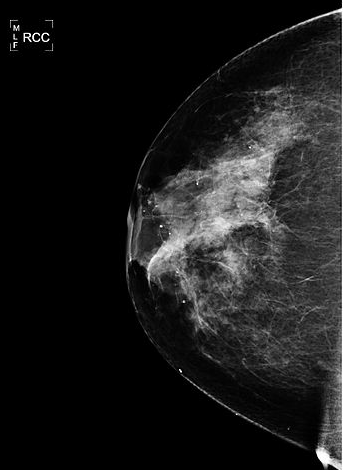
\includegraphics[width=3cm]{images/mammogram}};
	\node[xshift=-3cm,yshift=0.8cm] at (current page.south east) {\footnotesize{\textit{Image source: Wikimedia Commons}}};
	\end{tikzpicture}

	%\footfullcite{}
	
\end{frame}

\note{
	\begin{itemize}
		\item Machine learning is a powerful approach for developing sophisticated, \\
			automatic, and objective models for the analysis of data
		\item Machine learning specifically promises to help physicians make better or faster diagnoses, ...
		\item ... choose the best medications for their patients, ...
		\item ... predict readmissions, ...
		\item ... identify patients at high-risk for poor outcomes, ...
		\item ... and in general improve patients' health while minimizing costs. 
	\end{itemize}

	\begin{itemize}
		\item you can find things with ML that you wouldn't be able to find otherwise
		\item many models today perform better than humans!
		\item a patient with a rare difficult condition can be matched to similar cases from the past
		\item faster diagnosis, better treatment
	\end{itemize}

	\begin{itemize}
		\item there is not really a place in medicine where AI doesn't have potential applications:
		\item more and more data is being collected that needs to be interpreted,
		\item meaning that diagnosis is increasingly data driven, e.g. in radiology.
		\item Moreover, ML allows the incorporation of data from heterogenous inputs: 
		\item clinical, genomics, drugs, electronic health records, etc.
		\item to predict e.g. drug responses, relapses, etc. for individual patients
		\item This way, ML will be a step towards personalized or precision medicine
	\end{itemize}
}

\note{	
	\begin{itemize}
		\item Examples for how ML is already being used in the medical field today come mainly from
		\item image recognition
		\item this is similar to training ML models to recognize images of cats (classification in images)
		\item This way, ML models can be trained to identify breast cancer, lung cancer, osteoporosis, brain tumors, etc. \\�from medical images
		\item With Computer-Aided Diagnosis (CAD), radiologists use the computer output as a 'second opinion' and make the final decisions
	\end{itemize}

	\begin{itemize}
		\item Another example is that facial analysis technology can help diagnose genetic disorders that often involve dysmorphic facial features, like trisomies
		\item Researchers at the University of Oxford in the United Kingdom have the developed
		\item Face2Gene, an app that uses machine learning.
		\item Doctors can upload a photo of patient's face to get a prediction for the type of genetic disorder he or she might have
	\end{itemize}

	\begin{itemize}
		\item What I want to mention at the end is that ML is not meant to replace medical professionals!
		\item Doctors are still important!
		\item But the computer will do the tasks that we humans are not good at, like interpreting complex images.
		\item Today, we already collect more data than humans can manage to make sense of (e.g. genomics data),
		\item so the clinicians will be freed up to think about best treatment options and talk more with the patients
		\item Moreover, good models are built on strong knowledge of the question and the biology behind it
		\item and features need to be evaluated in context
	\end{itemize}
}


%%%%%%%%%%%%%%%%%%%%%
%	SECTION
%	What makes a model meaningful?
%%%%%%%%%%%%%%%%%%%%%

\section{What makes a model meaningful?}

\begin{frame}
	
	\begin{center}
		\usebeamerfont*{frametitle} \usebeamercolor[fg]{frametitle} {\Huge{\textbf{Can we trust \\ \vspace{0.3cm} ML  models?}}}
	\end{center}
	
	\vspace{0.5cm}
	
	\begin{itemize}
		\item most ML algorithms model high-degree interactions \\ between variables 
		\item ML models are hard (or impossible) to interpret!
		\item we often don't know \alert{WHY} they make decisions
	\end{itemize}
	
	\begin{itemize}
		\item therefore, it is crucial that our models are \alert{meaningful}
	\end{itemize}
	
	\begin{tikzpicture}[remember picture,overlay]
	\node[xshift=-2.2cm,yshift=-1.5cm] at (current page.north east) {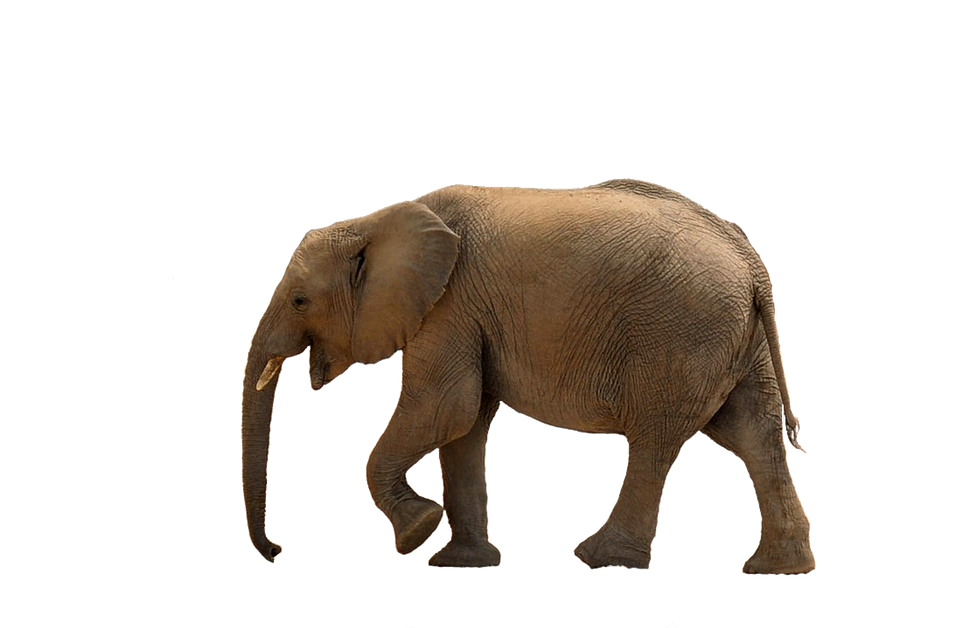
\includegraphics[width=5cm]{images/elephant}};
	\node[xshift=-2cm,yshift=-8.8cm] at (current page.north east) {\footnotesize{\textit{Image source: Pixabay}}};
	\end{tikzpicture}
\end{frame}

\note{
	\begin{itemize}
		\item I want to begin with the arguably central question concerning ML:
		\item Can we trust them?
		\item I consider this kind of the elephant in the room when we hear all the amazing things that ML models can do, like how they beat doctors in diagnosing cancers, etc.
		\item And when we test models on known data, it is easy to be wowed by high prediction accuracy. 
		\item But what we really want, is to be able to deploy our models to truly unknown data and still be confident that we can trust them
		\item Trust is not an easy thing to achieve, because the inherent problem with ML models is that they are hard (or impossible) to interpret
		\item This is because ML algorithms model high-degree interactions between variables 
		\item meaning the effect of combining many variables together
		\item This way, they tend to create nonlinear, 
		\item non-monotonic, 
		\item non-polynomial, 
		\item and even non-continuous functions 
		\item that approximate the relationship between independent and dependent variables in a data set
		\item This complexity, which bestows the extraordinary predictive abilities on machine learning algorithms also makes the answers these algorithms produce difficult (or even impossible) to understand.
		\item and we humans, especially non-experts in modeling, will have a hard time trusting a model that they don't understand
		\item difficulties in interpretation still present maybe the biggest barrier for the widespread, practical use of ML in clinical settings
	\end{itemize}
}

\note{	
	\begin{itemize}
		\item So, when working with data we should be asking ourselves some very hard questions: 
		\item do I understand my data? 
		\item Do I understand the model and the answers my machine learning algorithm is giving me? 
		\item And do I trust these answers? 
		\item trusting models and results is a general requirement for good (data) science
		\item so we need to make sure, that we are modeling is actually meaningful
	\end{itemize}
}

\begin{frame}
	\frametitle{What makes a model meaningful?}
	
	\begin{itemize}
		\item creating ML models is relatively easy
		\item creating \alert{good or meaningful} models is hard
	\end{itemize}
	
	\vspace{0.2cm}
	\alert{\textsl{Meaningful} models}
	\vspace{0.2cm}
	
	\begin{itemize}
		\item are generalizable
		\item answer the question(s) posed...
		\item ... with sufficient accuracy to be trustworthy
	\end{itemize}
	
	\vspace{0.2cm}
	
	\begin{center}
		{\Large \alert{Accuracy depends on the problem!}}
		
		\vspace{0.5cm}
		
		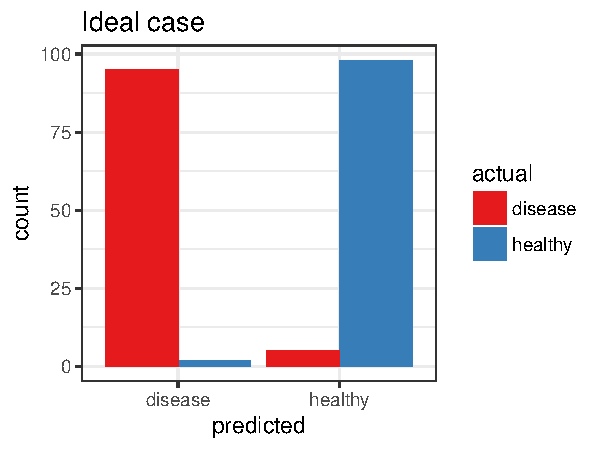
\includegraphics[width=0.33\textwidth]{images/meaningful_1}
		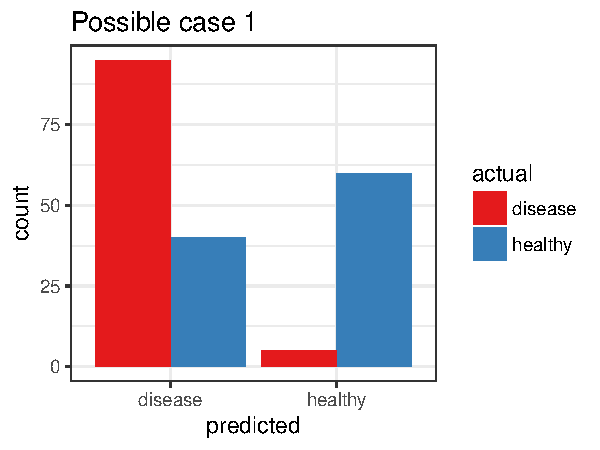
\includegraphics[width=0.33\textwidth]{images/meaningful_2}
		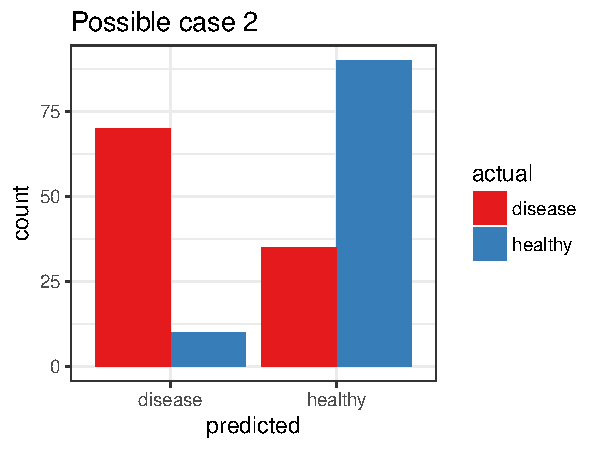
\includegraphics[width=0.33\textwidth]{images/meaningful_3}
	\end{center}
	
\end{frame}

\note{
	\begin{itemize}
		\item So, what makes a model 'meaningful'?
		\item With a little bit of practice, most anybody can build machine learning models.
		\item What is hard though, is to build 'good' or 'meaningful' models
	\end{itemize}
	
	\begin{enumerate}
		\item This means that the model needs to be generalizable, i.e. it needs to perform well on unseen data
		\item It needs to answer a \textbf{specific} question or address a specific problem, \\
		e.g. does a mammogram image show a healthy breast or is there a tumor? \\
		Or does an ECG show a normal heart rhythm or arrhythmia?
		\item And it needs to produce a correct prediction (such as a diagnosis) with high enough accuracy that we trust it!
	\end{enumerate}
	
	\begin{itemize}
		\item We therefore need to evaluate model accuracy when we want to establish ML for a specific task
		\item before we can decide whether it is trustworthy enough to implement in real-life, 
		\item like in a hospital where it could e.g. assist doctors in making decisions about treatment
	\end{itemize}
	
	\begin{itemize}
		\item But what exactly denotes a \textsl{high enough accuracy} can not be defined with a one-size-fits-all approach: 
		\item accuracy depends on the problem we want to model because	
		\item a model needs to perform well in the real world, not in the lab on training data
	\end{itemize}
}

\note{
	Let me illustrate what I mean with the following examples:
	\begin{itemize}
		\item \alert{Ideal case:} Of course, we all want to achieve ideal modeling results where overall prediction accuracy is very high. \\ 
		With a model like that, we can be very confident that a healthy person is indeed healthy and a sick person is not. \\
		\item But in reality, we often achieve prediction accuracies that are much less nice. \\
		\item \alert{Scenarios 1 and 2:} Le's consider two possible scenarios: 
		\item in scenario 1, we can be very confident that a person who got classified as "healthy" is indeed healthy, \\ 
		while a person who has been diagnosed as diseased might as well be healthy based on these prediction accuracies
		\item in case 2, it is the other way around.
		\item We now need to make a decision which scenario is better and in which direction we want to optimize our model: \\ 
		do we rather want to refer a few healthy people for further checking because the model predicted them as diseased? \\ 
		Or do we rather want to be as certain as possible that a predicted disease is actually true \\ 
		and accept that we might miss a few disease cases?
	\end{itemize}
}

%%%%%%%%%%%%%%%%%%%%%
%	SECTION
%	A quick recap of ML basics
%%%%%%%%%%%%%%%%%%%%%

\section{A quick recap of ML basics}

\begin{frame}
	\frametitle{Machine learning}

	\begin{itemize}
		\item artificial intelligence (AI)
		\item data-driven
		\item algorithms \alert{learn} by being trained on observed data...
		\item ... and \alert{predict unknown data}
		\item the increase in computational capacity has made ML more accessible
	\end{itemize}
	
	\begin{block} {}	
		\begin{center}
			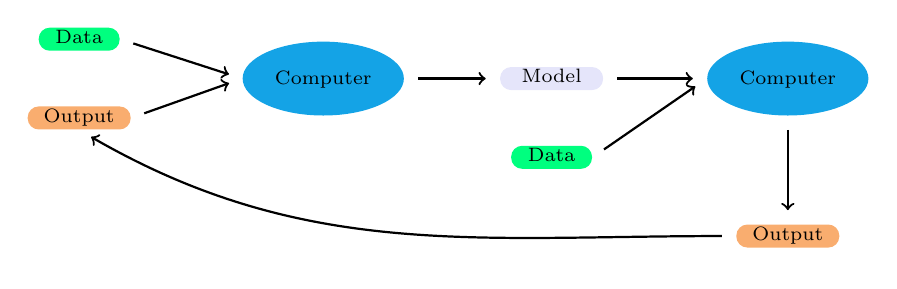
\begin{tikzpicture}
			\scriptsize
			\node[rectangle, rounded corners, text height=1ex,text depth=0ex,align=center,text width=3em,text centered,minimum height=1em, fill = SpringGreen] (Data) at (0,0) {Data};
			\node[rectangle, rounded corners, text height=1ex,text depth=0ex,align=center,text width=4em,text centered,minimum height=1em, fill = Lavender] (Model) at (6,-0.5) {Model};
			\node[ellipse, text height=3ex,text depth=1.5ex,align=center,text width=4.5em,text centered,minimum height=3em, fill = Cerulean] (Computer) at (3.1,-0.5) {Computer};
			\node[rectangle, rounded corners, text height=1ex,text depth=0ex,align=center,text width=4em,text centered,minimum height=1em, fill = Apricot] (Output) at (0,-1) {Output};
			\node[ellipse, text height=3ex,text depth=1.5ex,align=center,text width=4.5em,text centered,minimum height=3em, fill = Cerulean] (Computer2) at (9,-0.5) {Computer};
			\node[rectangle, rounded corners, text height=1ex,text depth=0ex,align=center,text width=4em,text centered,minimum height=1em, fill = Apricot] (Output2) at (9,-2.5) {Output};
			\node[rectangle, rounded corners, text height=1ex,text depth=0ex,align=center,text width=3em,text centered,minimum height=1em, fill = SpringGreen] (Data2) at (6,-1.5) {Data};
			
			\draw[->,thick,shorten >=5pt,shorten <=5pt] (Data.east) -- (Computer.west);
			\draw[->,thick,shorten >=5pt,shorten <=5pt] (Output.east) -- (Computer.west);
			\draw[->,thick,shorten >=5pt,shorten <=5pt] (Computer.east) -- (Model.west);
			\draw[->,thick,shorten >=5pt,shorten <=5pt] (Model.east) -- (Computer2.west);
			\draw[->,thick,shorten >=5pt,shorten <=5pt] (Computer2.south) -- (Output2.north);
			\draw[->,thick,shorten >=5pt,shorten <=5pt] (Data2.east) -- (Computer2.west);
			\draw[->,thick,shorten >=5pt,shorten <=5pt] (Output2.west) to [out=180,in=330] (Output.south);
			\end{tikzpicture}
		\end{center}
	\end{block}
\end{frame}

\note{
	\begin{itemize}
		\item ML is a subfield of computer science
		\item that falls in the general category of AI
		\item In ML, algorithms learn models from known data
		\item and are then able to use this inferred knowledge for predicting unknown data 
		\item ML concepts are not new, but the increase in computational capacity and the bigger amounts of data that we are able to collect in shorter periods of time, has made them more accessible and applicable
	\end{itemize}
}

\begin{frame}
	\frametitle{Supervised vs Unsupervised learning}

	\begin{columns}
		
		\column{0.5\textwidth}
	
	\begin{block}{}
		\centering
		\alert{Supervised}
	\end{block}

	\begin{center}
		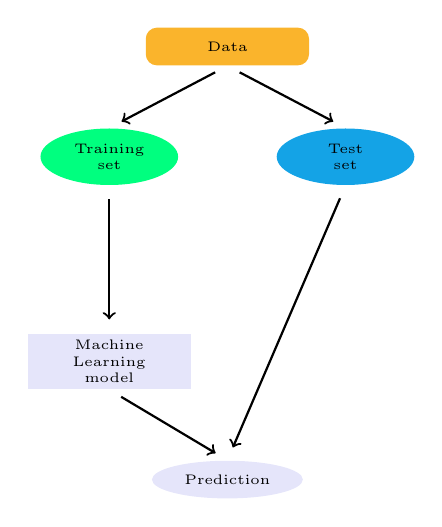
\begin{tikzpicture}
		\tiny
		\node[rectangle, rounded corners, align=center,text width=8em,text centered,minimum height=2em, fill = Dandelion] (select) at (2.5,-3) {Data};
		
		\node[ellipse,align=center,text width=4.5em,text centered,minimum height=3em, fill = SpringGreen] (training) at (1,-4.4) {Training set};
		
		\node[ellipse,align=center,text width=4.5em,text centered,minimum height=3em, fill = Cerulean] (test) at (4,-4.4) {Test \\ set};
		
		\node[rectangle, align=center,text width=8em,text centered,minimum height=2em, fill = Lavender] (rf) at (1,-7.0) {Machine \\ Learning \\ model};
		
		\node[ellipse,align=center,text width=5em,text centered,minimum height=2em, fill = Lavender] (prediction) at (2.5,-8.5) {Prediction};
		
		\draw[->,thick,shorten >=5pt,shorten <=5pt] (select.south) -- (training.north);
		\draw[->,thick,shorten >=5pt,shorten <=5pt] (select.south) -- (test.north);
		
		\draw[->,thick,shorten >=5pt,shorten <=5pt] (training.south) -- (rf.north);
		\draw[->,thick,shorten >=5pt,shorten <=5pt] (test.south) -- (prediction.north);
		
		\draw[->,thick,shorten >=5pt,shorten <=5pt] (rf.south) -- (prediction.north);
		\end{tikzpicture}
		
		\footnotesize{\textit{}}
	\end{center}

	\column{0.5\textwidth}
	
	\begin{block}{}
		\centering
		\alert{Unsupervised}
	\end{block}

	\centering
	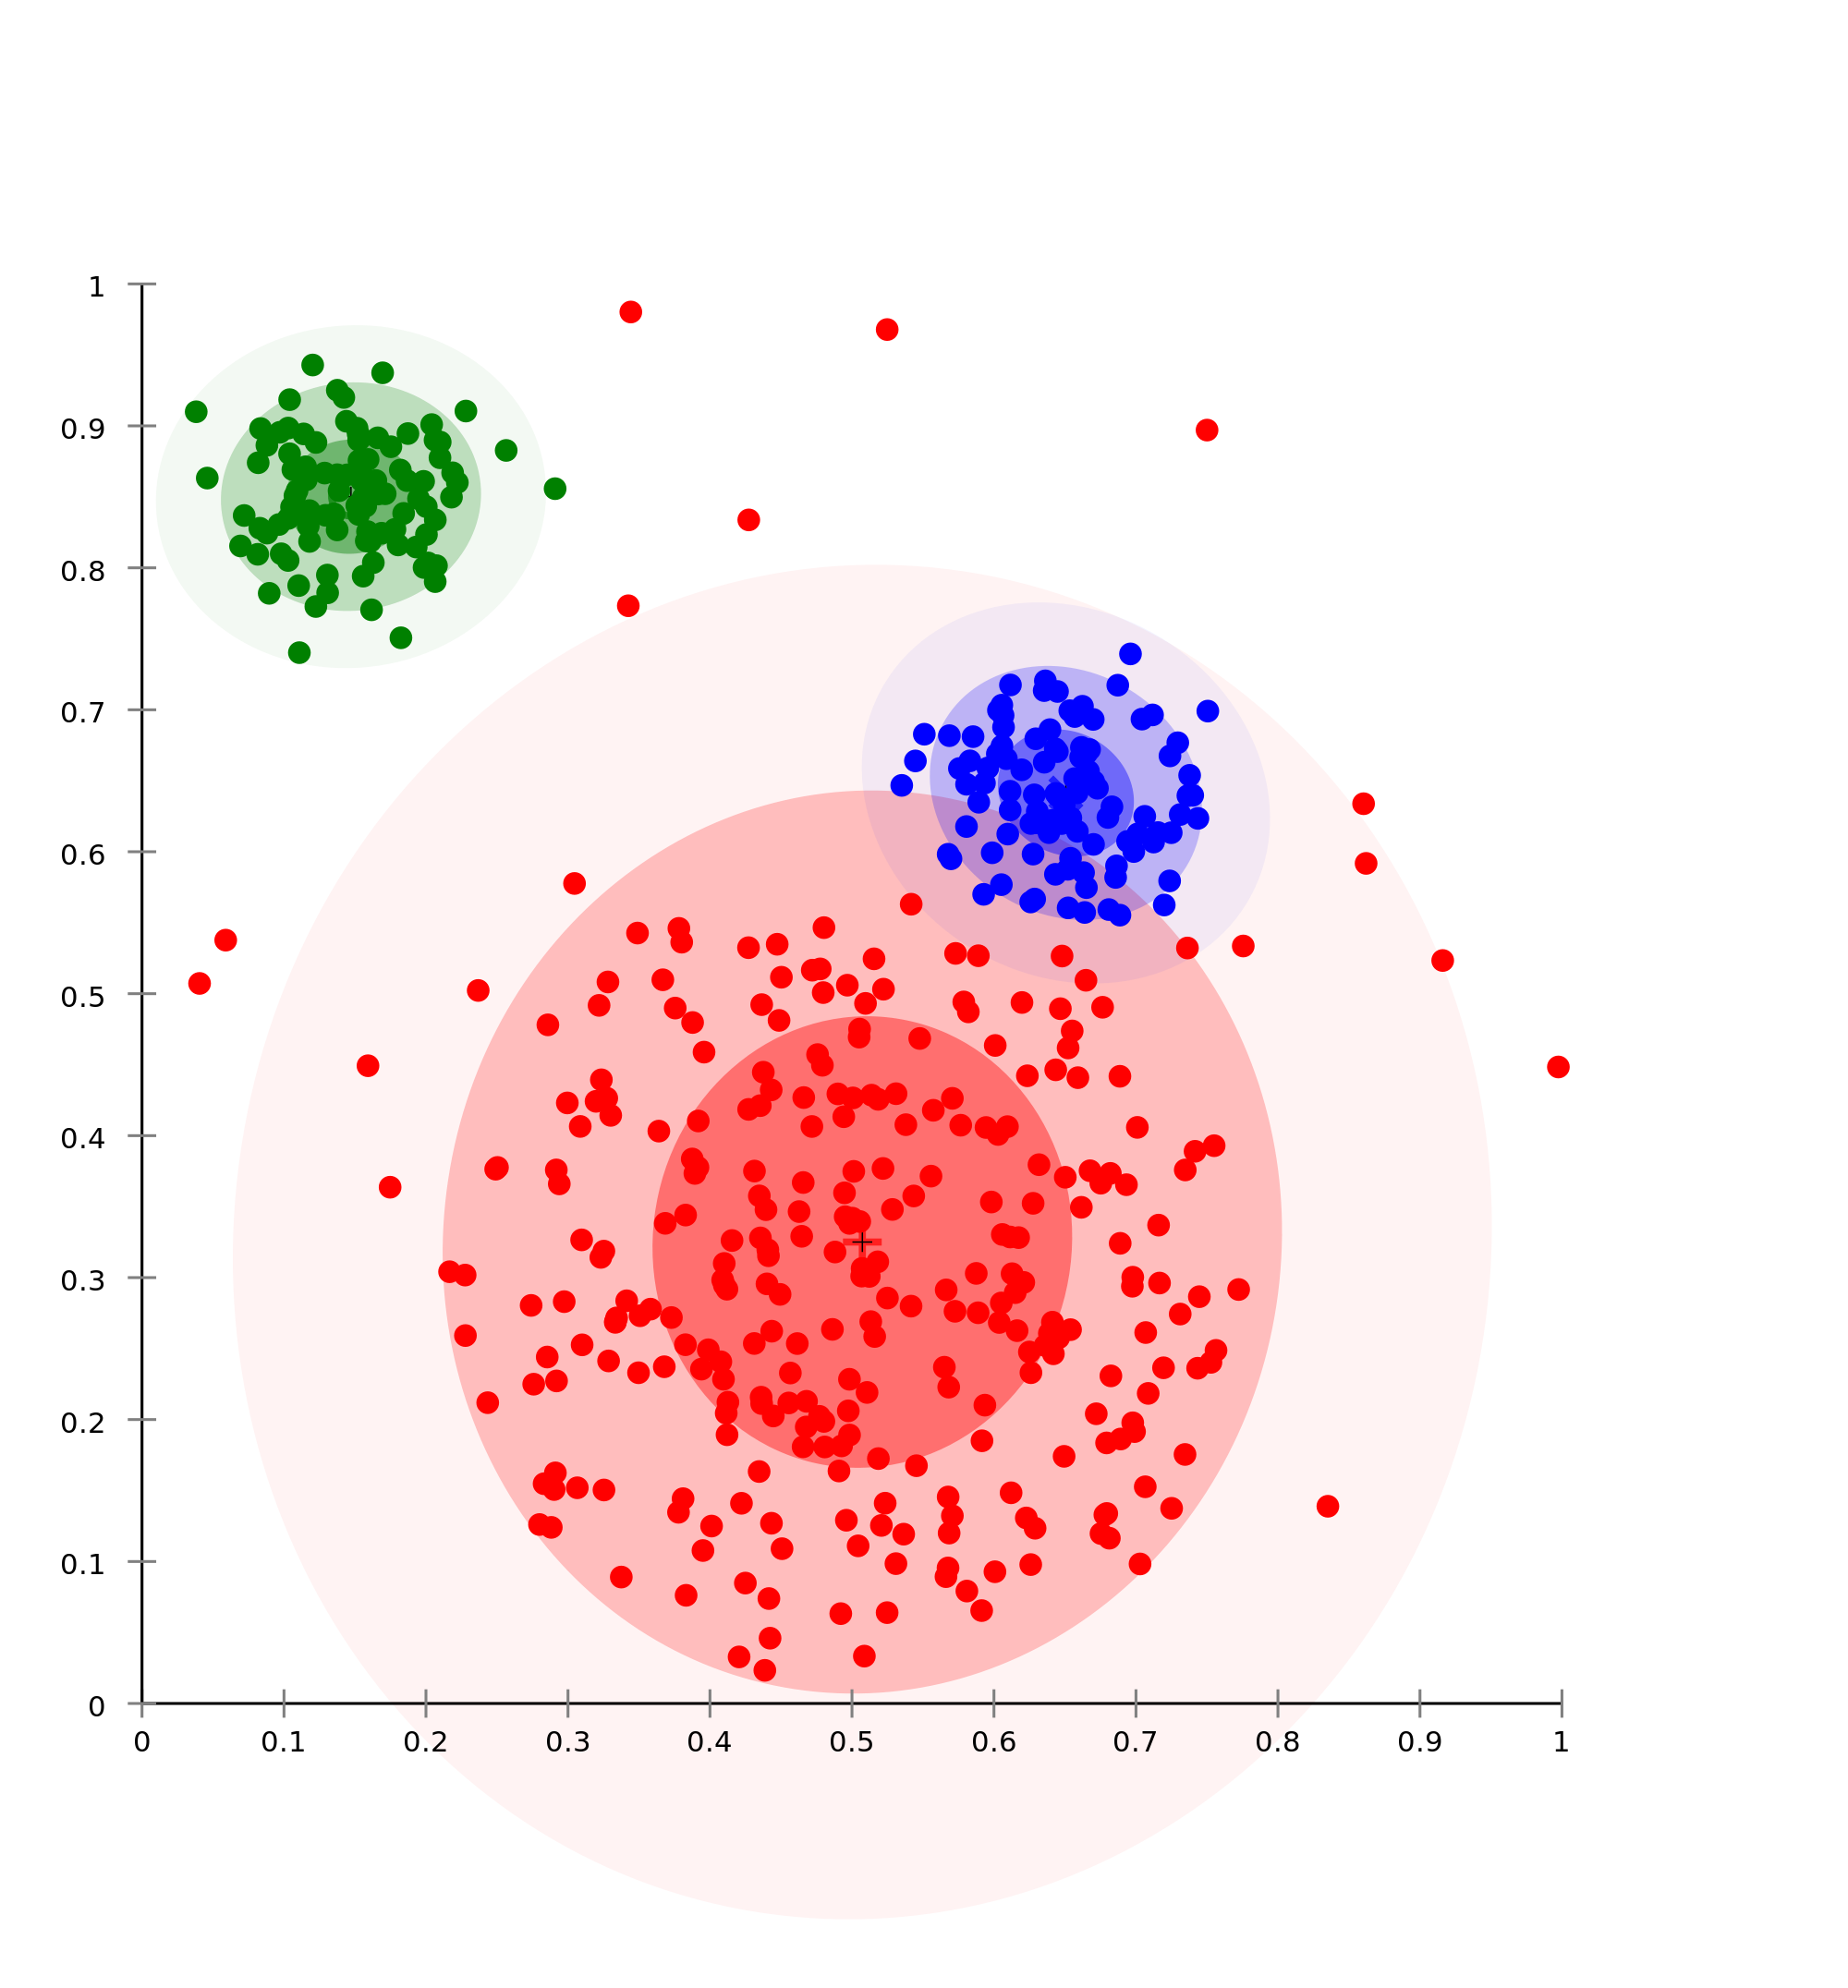
\includegraphics[width=0.5\textwidth]{images/clustering1}
	
	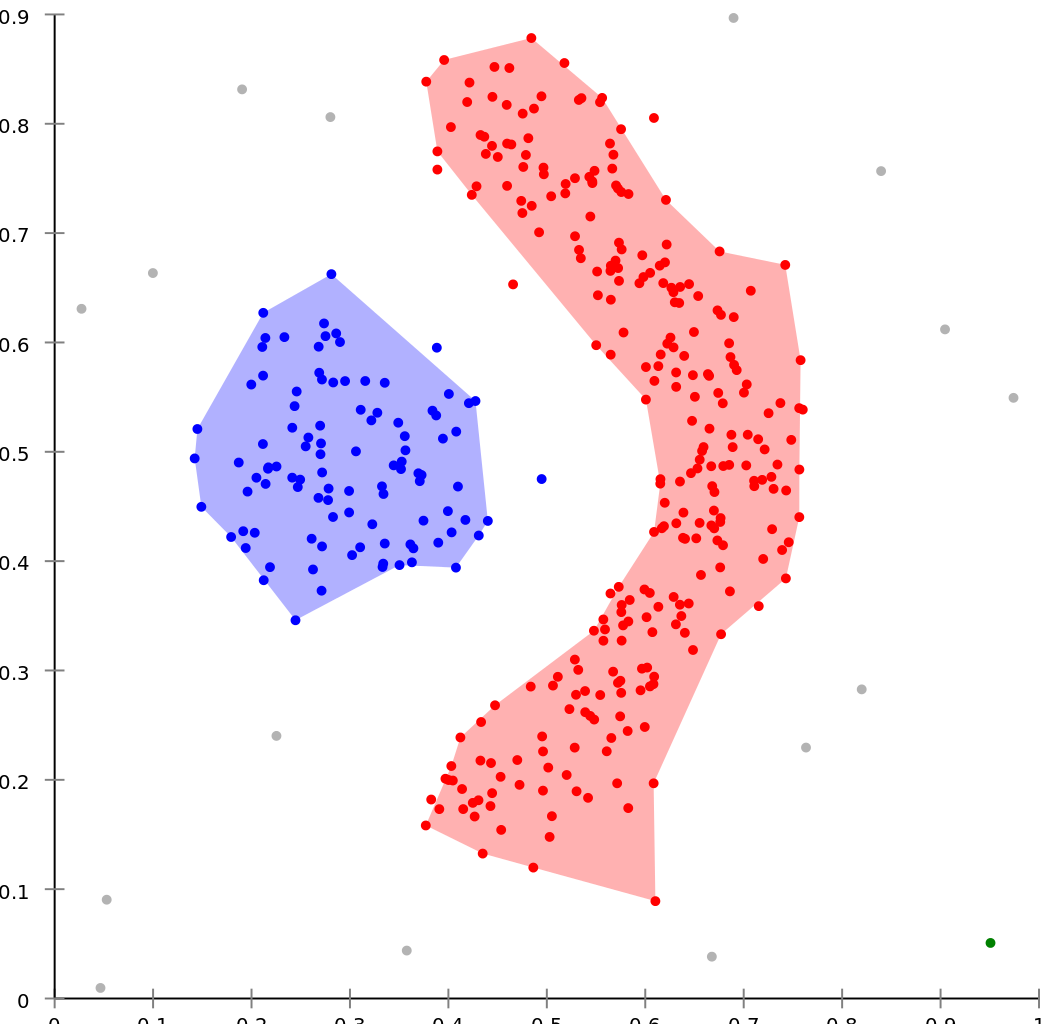
\includegraphics[width=0.5\textwidth]{images/clustering2}
	
	\footnotesize{\textit{Image Source: Wikipedia}}
	
	\end{columns}
\end{frame}

\note{
	\begin{itemize}
		\item ML is generally divided into two categories: Supervised and unsupervised
		\item even though there are also hybrid methods, called semi-supervised
	\end{itemize}

	\begin{itemize}
		\item In supervised learning,
		\item classification labels are assigned to each training sample
		\item these labels are then used as output variables for the model
		\item Examples are SVM or decision trees
	\end{itemize}
	
	\begin{itemize}
		\item Unsupervised learning on the other hand does not require an input, like class lables
		\item Methods, like matrix decomposition, e.g. nonnegative matrix factorization
		\item basically perform pattern recognition and 
		\item cluster similar data points into groups
	\end{itemize}

	\begin{itemize}
	\item Semi-supervised methods require a little bit of input, like how many clusters or classes to find in the data
	\end{itemize}

	Here, I will focus on supervised learning!
}


\begin{frame}
	\frametitle{Classification vs Regression}

		\begin{columns}
		
		\column{0.5\textwidth}
		
				\begin{block}{}
			\centering
			\alert{Regression} \\
			e.g. weight loss
		\end{block}
		
		\begin{center}
			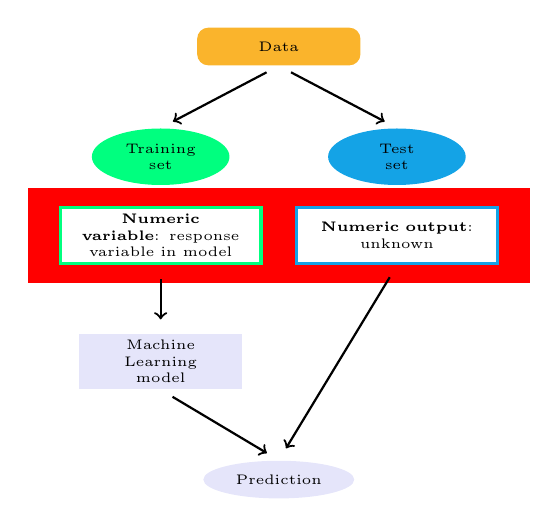
\begin{tikzpicture}
			\tiny
			\node[rectangle, rounded corners, align=center,text width=8em,text centered,minimum height=2em, fill = Dandelion] (select) at (2.5,-3) {Data};
			
			\node[ellipse,align=center,text width=4.5em,text centered,minimum height=3em, fill = SpringGreen] (training) at (1,-4.4) {Training set};
			
			\node[rectangle, align=center,text width=26em,text centered,minimum height=5em, fill = Red] () at (2.5,-5.4) {};
			
			\node[rectangle, align=center,text width=10em,text centered,minimum height=3em, draw = SpringGreen, very thick, fill = White] (class1) at (1,-5.4) {\textbf{Numeric \\ variable}: response variable in model};
			
			\node[ellipse,align=center,text width=4.5em,text centered,minimum height=3em, fill = Cerulean] (test) at (4,-4.4) {Test \\ set};
			
			\node[rectangle, align=center,text width=10em,text centered,minimum height=3em, draw = Cerulean, very thick, fill = White] (class2) at (4,-5.4) {\textbf{Numeric output}: \\ unknown};
			
			\node[rectangle, align=center,text width=8em,text centered,minimum height=2em, fill = Lavender] (rf) at (1,-7.0) {Machine \\ Learning \\ model};
			
			\node[ellipse,align=center,text width=5em,text centered,minimum height=2em, fill = Lavender] (prediction) at (2.5,-8.5) {Prediction};
			
			\draw[->,thick,shorten >=5pt,shorten <=5pt] (select.south) -- (training.north);
			\draw[->,thick,shorten >=5pt,shorten <=5pt] (select.south) -- (test.north);
			
			\draw[->,thick,shorten >=5pt,shorten <=5pt] (class1.south) -- (rf.north);
			\draw[->,thick,shorten >=5pt,shorten <=5pt] (class2.south) -- (prediction.north);
			
			\draw[->,thick,shorten >=5pt,shorten <=5pt] (rf.south) -- (prediction.north);
			\end{tikzpicture}
		\end{center}
		
		\column{0.5\textwidth}
		
		\pause
		
		\begin{block}{}
			\centering
			\alert{Classification} \\
			e.g. healthy vs disease
		\end{block}
		
		\begin{center}
			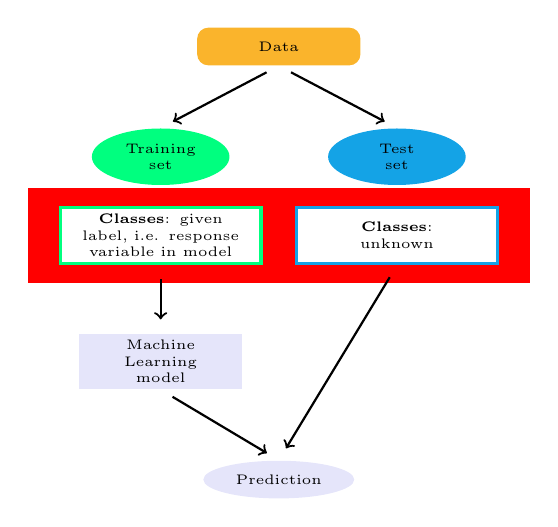
\begin{tikzpicture}
			\tiny
			\node[rectangle, rounded corners, align=center,text width=8em,text centered,minimum height=2em, fill = Dandelion] (select) at (2.5,-3) {Data};
			
			\node[ellipse,align=center,text width=4.5em,text centered,minimum height=3em, fill = SpringGreen] (training) at (1,-4.4) {Training set};
			
			\node[rectangle, align=center,text width=26em,text centered,minimum height=5em, fill = Red] () at (2.5,-5.4) {};
			
			\node[rectangle, align=center,text width=10em,text centered,minimum height=3em, draw = SpringGreen, very thick, fill = White] (class1) at (1,-5.4) {\textbf{Classes}: given label, i.e. response variable in model};
			
			\node[ellipse,align=center,text width=4.5em,text centered,minimum height=3em, fill = Cerulean] (test) at (4,-4.4) {Test \\ set};
			
			\node[rectangle, align=center,text width=10em,text centered,minimum height=3em, draw = Cerulean, very thick, fill = White] (class2) at (4,-5.4) {\textbf{Classes}: \\ unknown};
			
			\node[rectangle, align=center,text width=8em,text centered,minimum height=2em, fill = Lavender] (rf) at (1,-7.0) {Machine \\ Learning \\ model};
			
			\node[ellipse,align=center,text width=5em,text centered,minimum height=2em, fill = Lavender] (prediction) at (2.5,-8.5) {Prediction};
			
			\draw[->,thick,shorten >=5pt,shorten <=5pt] (select.south) -- (training.north);
			\draw[->,thick,shorten >=5pt,shorten <=5pt] (select.south) -- (test.north);
			
			\draw[->,thick,shorten >=5pt,shorten <=5pt] (class1.south) -- (rf.north);
			\draw[->,thick,shorten >=5pt,shorten <=5pt] (class2.south) -- (prediction.north);
			
			\draw[->,thick,shorten >=5pt,shorten <=5pt] (rf.south) -- (prediction.north);
			\end{tikzpicture}
		\end{center}
		
	\end{columns}
\end{frame}

\note{
	\begin{itemize}
		\item Within supervised learning, the two main task are classification and regression.
		\item Let's say your learning algorithm seeks a function that predicts a response variable from input variables. 
		\item If the response variable is expressed as classes, it is a classification problem. 
		\item Alternatively, if the response variable space is continuous, it is a regression problem.
	\end{itemize}

	\begin{itemize}
		\item Functions created by linear regression algorithms are probably the most interpretable class of models.
		\item For this reason, linear models were the go-to applied predictive modeling tool for decades, 
		\item even though this usually meant obtaining a somewhat lower accuracy could have been achieved with more complex models.
		\item In linear models, for every change in any given independent variable, the response function changes at a defined rate, 
		\item in only one direction, and at a magnitude represented by a readily available coefficient
	\end{itemize}

	\begin{itemize}
		\item Most machine learning algorithms however, create nonlinear response functions. 
		\item These more complex models are the most difficult to interpret, because they can change in a positive and negative direction and at a varying rate for any change in an independent variable. 
		\item Typically, the only standard interpretability measure these functions provide are relative variable importance measures
	\end{itemize}
}


\begin{frame}
	\frametitle{Features}
	
	\begin{columns}
		\column{0.5\textwidth}
	
	\begin{itemize}
	\item variables used for model training.
	\item using the right features is crucial.
	\end{itemize}

		\vspace{0.5cm}

	\begin{itemize}
		\item \alert{More is not necessarily better (overfitting)!}
	\end{itemize}
	
		\vspace{0.5cm}

	\begin{itemize}
		\item feature selection
		\item feature extraction/ engineering
	\end{itemize}

	\column{0.5\textwidth}
	\begin{tikzpicture}[remember picture,overlay]
	\node[xshift=-3cm,yshift=4.5cm] at (current page.south east) {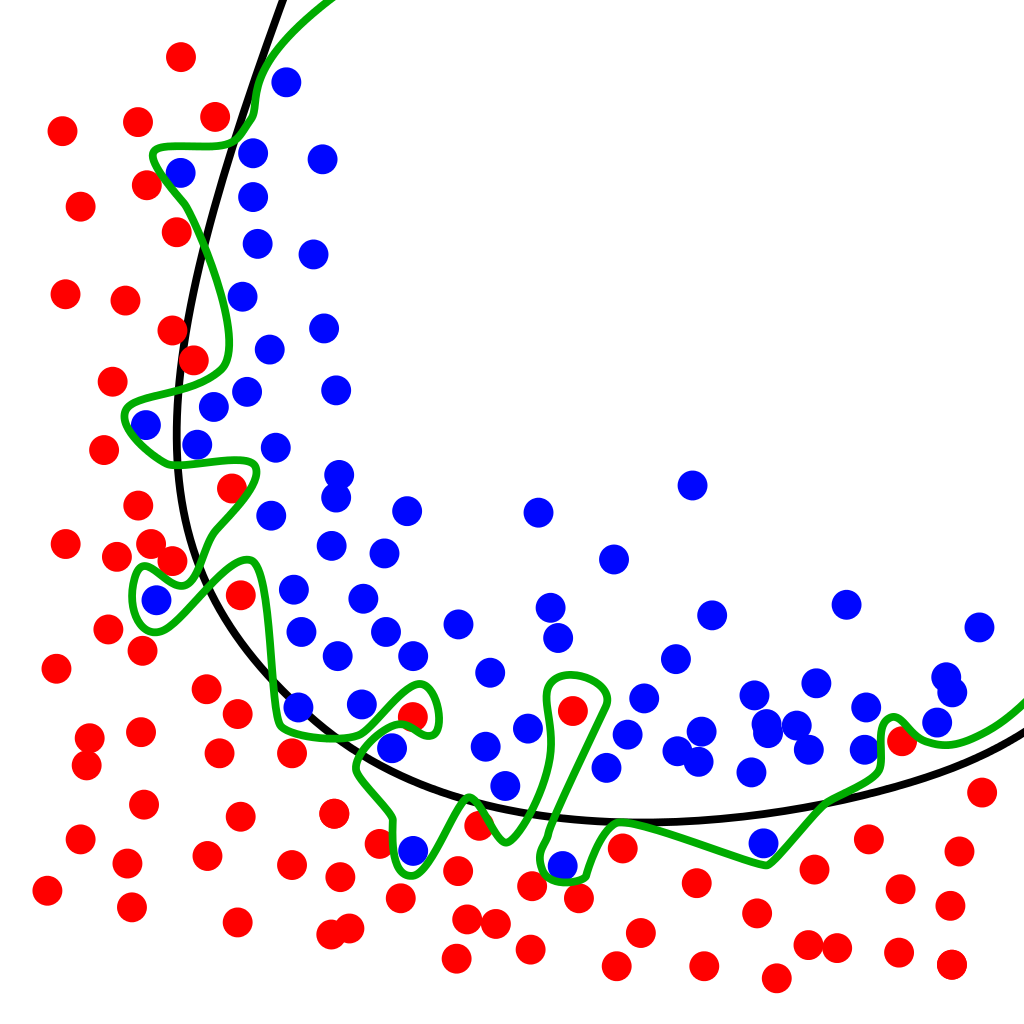
\includegraphics[width=5cm]{images/Overfitting}};
	\node[xshift=-2.5cm,yshift=1.5cm] at (current page.south east) {{\footnotesize \textit{Image Source: Wikipedia}}};
	\end{tikzpicture}
	
	\end{columns}
\end{frame}

\note{
	\begin{itemize}
		\item Machine learning uses so called features (sometimes also called variables or attributes) to generate predictive models
		\item Using a suitable combination of features is essential for obtaining high accuracy. 
		\item Because too many (unspecific) features pose the problem of overfitting the model, we generally want to restrict the features in our models to those, that are most relevant for the response variable we want to predict. 
		\item Using as few features as possible will also reduce the complexity of our models, which means it needs less time and computer power to run and is easier to understand. 
		\item Sometimes extraction of salient structure in the data that is more informative than the raw data itself 		\item this describes the feature extraction or feature engineering problem
	\end{itemize}
}

\begin{frame}
	\frametitle{Training, cross-validation and test data}
	
	\begin{center}
		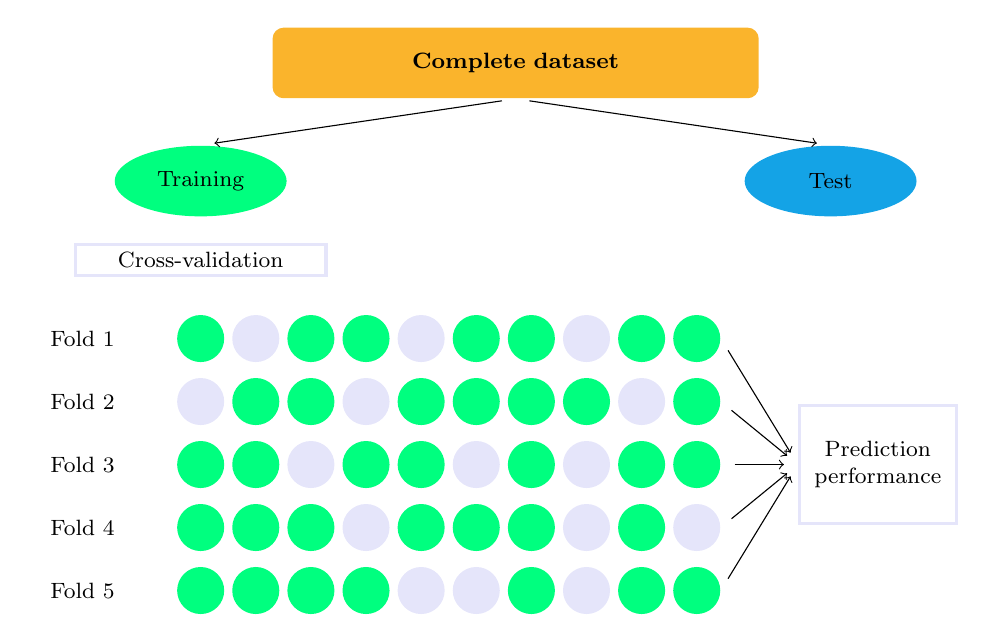
\begin{tikzpicture}
		\footnotesize
		
		\node[rectangle, rounded corners, align=center,text width=20em,text centered,minimum height=3em, fill = Dandelion] (data) at (4, 3.5) {\textbf{Complete dataset}};
		
		\node[ellipse,align=center,text width=4.5em,text centered,minimum height=3em, fill = SpringGreen] (train) at (0,2) {Training};
		
		\node[ellipse,align=center,text width=4.5em,text centered,minimum height=3em, fill = Cerulean] (test) at (8,2) {Test};
		
		\draw[->,shorten >=5pt,shorten <=5pt] (data.south) -- (train.north);
		\draw[->,shorten >=5pt,shorten <=5pt] (data.south) -- (test.north);
		
		\node[rectangle, align=center,text width=10em,text centered,minimum height=1em, draw = Lavender, very thick] () at (0,1) {Cross-validation};
		
		\node[rectangle, align=center,text width=4em,text centered,minimum height=1em] () at (-1.5, 0) {Fold 1};
		\node[ellipse, fill = SpringGreen, minimum height=2em, minimum width=2em] () at (0,0) {};
		\node[ellipse, fill = Lavender, minimum height=2em, minimum width=2em] () at (0.7,0) {};
		\node[ellipse, fill = SpringGreen, minimum height=2em, minimum width=2em] () at (1.4,0) {};
		\node[ellipse, fill = SpringGreen, minimum height=2em, minimum width=2em] () at (2.1,0) {};
		\node[ellipse, fill = Lavender, minimum height=2em, minimum width=2em] () at (2.8,0) {};
		\node[ellipse, fill = SpringGreen, minimum height=2em, minimum width=2em] () at (3.5,0) {};
		\node[ellipse, fill = SpringGreen, minimum height=2em, minimum width=2em] () at (4.2,0) {};
		\node[ellipse, fill = Lavender, minimum height=2em, minimum width=2em] () at (4.9,0) {};
		\node[ellipse, fill = SpringGreen, minimum height=2em, minimum width=2em] () at (5.6,0) {};
		\node[ellipse, fill = SpringGreen, minimum height=2em, minimum width=2em] (f1) at (6.3,0) {};
		
		\node[rectangle, align=center,text width=4em,text centered,minimum height=1em] () at (-1.5, -0.8) {Fold 2};
		\node[ellipse, fill = Lavender, minimum height=2em, minimum width=2em] () at (0,-0.8) {};
		\node[ellipse, fill = SpringGreen, minimum height=2em, minimum width=2em] () at (0.7,-0.8) {};
		\node[ellipse, fill = SpringGreen, minimum height=2em, minimum width=2em] () at (1.4,-0.8) {};
		\node[ellipse, fill = Lavender, minimum height=2em, minimum width=2em] () at (2.1,-0.8) {};
		\node[ellipse, fill = SpringGreen, minimum height=2em, minimum width=2em] () at (2.8,-0.8) {};
		\node[ellipse, fill = SpringGreen, minimum height=2em, minimum width=2em] () at (3.5,-0.8) {};
		\node[ellipse, fill = SpringGreen, minimum height=2em, minimum width=2em] () at (4.2,-0.8) {};
		\node[ellipse, fill = SpringGreen, minimum height=2em, minimum width=2em] () at (4.9,-0.8) {};
		\node[ellipse, fill = Lavender, minimum height=2em, minimum width=2em] () at (5.6,-0.8) {};
		\node[ellipse, fill = SpringGreen, minimum height=2em, minimum width=2em] (f2) at (6.3,-0.8) {};
		
		\node[rectangle, align=center,text width=4em,text centered,minimum height=1em] () at (-1.5, -1.6) {Fold 3};
		\node[ellipse, fill = SpringGreen, minimum height=2em, minimum width=2em] () at (0,-1.6) {};
		\node[ellipse, fill = SpringGreen, minimum height=2em, minimum width=2em] () at (0.7,-1.6) {};
		\node[ellipse, fill = Lavender, minimum height=2em, minimum width=2em] () at (1.4,-1.6) {};
		\node[ellipse, fill = SpringGreen, minimum height=2em, minimum width=2em] () at (2.1,-1.6) {};
		\node[ellipse, fill = SpringGreen, minimum height=2em, minimum width=2em] () at (2.8,-1.6) {};
		\node[ellipse, fill = Lavender, minimum height=2em, minimum width=2em] () at (3.5,-1.6) {};
		\node[ellipse, fill = SpringGreen, minimum height=2em, minimum width=2em] () at (4.2,-1.6) {};
		\node[ellipse, fill = Lavender, minimum height=2em, minimum width=2em] () at (4.9,-1.6) {};
		\node[ellipse, fill = SpringGreen, minimum height=2em, minimum width=2em] () at (5.6,-1.6) {};
		\node[ellipse, fill = SpringGreen, minimum height=2em, minimum width=2em] (f3) at (6.3,-1.6) {};
		
		\node[rectangle, align=center,text width=4em,text centered,minimum height=1em] () at (-1.5, -2.4) {Fold 4};
		\node[ellipse, fill = SpringGreen, minimum height=2em, minimum width=2em] () at (0,-2.4) {};
		\node[ellipse, fill = SpringGreen, minimum height=2em, minimum width=2em] () at (0.7,-2.4) {};
		\node[ellipse, fill = SpringGreen, minimum height=2em, minimum width=2em] () at (1.4,-2.4) {};
		\node[ellipse, fill = Lavender, minimum height=2em, minimum width=2em] () at (2.1,-2.4) {};
		\node[ellipse, fill = SpringGreen, minimum height=2em, minimum width=2em] () at (2.8,-2.4) {};
		\node[ellipse, fill = SpringGreen, minimum height=2em, minimum width=2em] () at (3.5,-2.4) {};
		\node[ellipse, fill = SpringGreen, minimum height=2em, minimum width=2em] () at (4.2,-2.4) {};
		\node[ellipse, fill = Lavender, minimum height=2em, minimum width=2em] () at (4.9,-2.4) {};
		\node[ellipse, fill = SpringGreen, minimum height=2em, minimum width=2em] () at (5.6,-2.4) {};
		\node[ellipse, fill = Lavender, minimum height=2em, minimum width=2em] (f4) at (6.3,-2.4) {};
		
		\node[rectangle, align=center,text width=4em,text centered,minimum height=1em] () at (-1.5, -3.2) {Fold 5};
		\node[ellipse, fill = SpringGreen, minimum height=2em, minimum width=2em] () at (0,-3.2) {};
		\node[ellipse, fill = SpringGreen, minimum height=2em, minimum width=2em] () at (0.7,-3.2) {};
		\node[ellipse, fill = SpringGreen, minimum height=2em, minimum width=2em] () at (1.4,-3.2) {};
		\node[ellipse, fill = SpringGreen, minimum height=2em, minimum width=2em] () at (2.1,-3.2) {};
		\node[ellipse, fill = Lavender, minimum height=2em, minimum width=2em] () at (2.8,-3.2) {};
		\node[ellipse, fill = Lavender, minimum height=2em, minimum width=2em] () at (3.5,-3.2) {};
		\node[ellipse, fill = SpringGreen, minimum height=2em, minimum width=2em] () at (4.2,-3.2) {};
		\node[ellipse, fill = Lavender, minimum height=2em, minimum width=2em] () at (4.9,-3.2) {};
		\node[ellipse, fill = SpringGreen, minimum height=2em, minimum width=2em] () at (5.6,-3.2) {};
		\node[ellipse, fill = SpringGreen, minimum height=2em, minimum width=2em] (f5) at (6.3,-3.2) {};
		
		\node[rectangle, align=center,text width=6em,text centered,minimum height=5em, draw = Lavender, very thick] (perf) at (8.6, -1.6) {Prediction performance};
		
		\draw[->,shorten >=5pt,shorten <=5pt] (f1.east) -- (perf.west);
		\draw[->,shorten >=5pt,shorten <=5pt] (f2.east) -- (perf.west);
		\draw[->,shorten >=5pt,shorten <=5pt] (f3.east) -- (perf.west);
		\draw[->,shorten >=5pt,shorten <=5pt] (f4.east) -- (perf.west);
		\draw[->,shorten >=5pt,shorten <=5pt] (f5.east) -- (perf.west);
		\end{tikzpicture}
	\end{center}
\end{frame}

\note{
	\begin{itemize}
		\item A central aspect of modeling is to make them generalizable and avoid overfitting
		\item to achieve this, we can want to train our model on a dataset that separate from a test set
		\item in addition, we can add cross-validation strategies to the modeling process itself
		\item CV means that the main training set is randomly subdivided into 2 sets:
		\item one for actual training and one for validation
		\item the model is then trained on the training subset and predictions on the validation-hold-out-set are used to calculate and accuracy score
		\item this process is repeated several times (e.g. 5-fold)
		\item the prediction performance of the cross-validation can be used to optimize modeling
	\end{itemize}
}

\begin{frame}[plain, c]
	
	\begin{center}
	\usebeamerfont*{frametitle} \usebeamercolor[fg]{frametitle} {\Huge \textbf{Take home messages:}}
	\end{center}

	\vspace{0.5cm}
	
	\begin{itemize}
		\item ML models learn on observed data
		\item and predict unknown data
	\end{itemize}

	\vspace{0.3cm}
	
	\begin{itemize}
		\item creating ML models is easy
		\item creating \alert{good} models is hard
	\end{itemize}

	\vspace{0.3cm}
	
	\alert{Meaningful} models
	\begin{itemize}
		\item answer specific questions
		\item are able to generalize to unseen data
		\item can be trusted
	\end{itemize}

	\begin{tikzpicture}[remember picture,overlay]
	\node[xshift=-2.5cm,yshift=5.8cm] at (current page.south east) {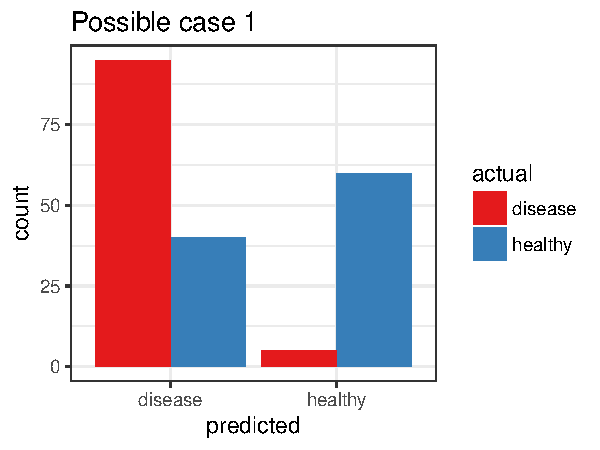
\includegraphics[width=0.4\textwidth]{images/meaningful_2}};
	\node[xshift=-2.5cm,yshift=2.1cm] at (current page.south east) {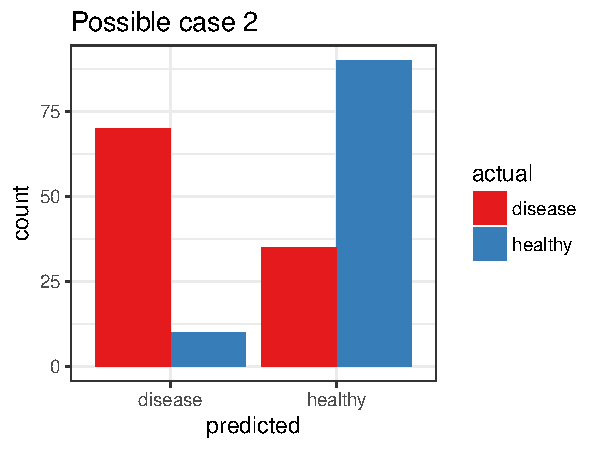
\includegraphics[width=0.4\textwidth]{images/meaningful_3}};
	\end{tikzpicture}
\end{frame}

\note{
	\begin{itemize}
		\item Here, I want to briefly summarize the most important aspects from my talk so far
		\item We will now look at a hands-on example of ML modeling in R
		\item When doing the actual work, I know from experience that it is easy to get caught up in the nitty gritty of writing code and trying out different things
		\item but I want to encourage you to try and not loose sight of the bigger picture
	\end{itemize}
}

%%%%%%%%%%%%%%%%%%%%%
%	SECTION
%	How to build ML models in R
%%%%%%%%%%%%%%%%%%%%%

\section{How to build ML models in R}

\begin{frame}
	\frametitle{Session setup}
	
	\begin{itemize}
		\item \href{http://archive.ics.uci.edu/ml/machine-learning-databases/breast-cancer-wisconsin/}{Breast Cancer Wisconsin Dataset}\footfullcite{Wolberg01121990} \\ \vspace{0.1cm}
		\includegraphics[height=2cm]{images/Needle_Biopsy.jpg}
		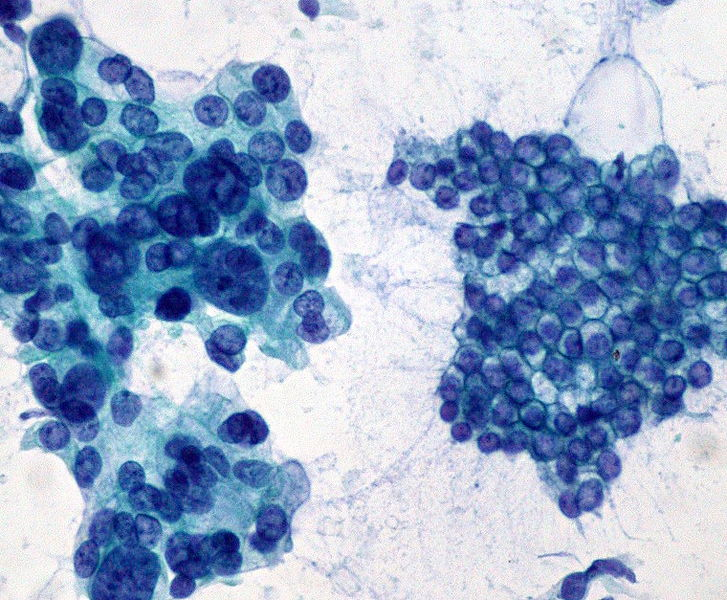
\includegraphics[height=2cm]{images/fna.jpg} \\
		\hspace{1.7cm} \footnotesize{\textit{Image Source: Wikipedia}} \vspace{0.1cm}
		\item caret\footfullcite{caret}
		\item h2o\footfullcite{h2o}
	\end{itemize}
	
	\vspace{0.3cm}
	
	\centering
	Code will be available on \href{https://shiring.github.io}{my website} and on \href{https://github.com/ShirinG/Webinar_ISDS}{Github}
	
	\begin{tikzpicture}[remember picture,overlay]
	\node[xshift=-2.3cm,yshift=-2.3cm] at (current page.north east) {
\includegraphics[width=3cm]{images/R_logo.png}};
	\end{tikzpicture}
	
\end{frame}

\note{
	\begin{itemize}
		\item First, a few words about the logistics:
		\item All analyses have been done in R 3.3.3 using RStudio 1.0.136
		\item As case study example, I am using the breast cancer dataset from Dr. William H. Wolberg of the University of Wisconsin Hospitals, Madison
	\end{itemize}
	
	\begin{itemize}
		\item It looks at the predictor classes:
		\item malignant or
		\item benign breast mass
	\end{itemize}
	
	\begin{itemize}
		\item The features characterise cell nucleus properties
		\item and were generated from image analysis of fine needle aspirates (FNA) of breast masses:
		\item Sample ID (code number)
		\item Clump thickness
		\item Uniformity of cell size
		\item Uniformity of cell shape
		\item Marginal adhesion
		\item Single epithelial cell size
		\item Number of bare nuclei
		\item Bland chromatin
		\item Number of normal nuclei
		\item Mitosis
		\item Classes, i.e. diagnosis
	\end{itemize}
}

\begin{frame}
	\frametitle{Get to know your data}
	
	\alert{Response variable}
	\begin{itemize}
		\item Is it balanced?
	\end{itemize}
	
	\begin{columns}	
		\column{0.5\textwidth}
		\centering
		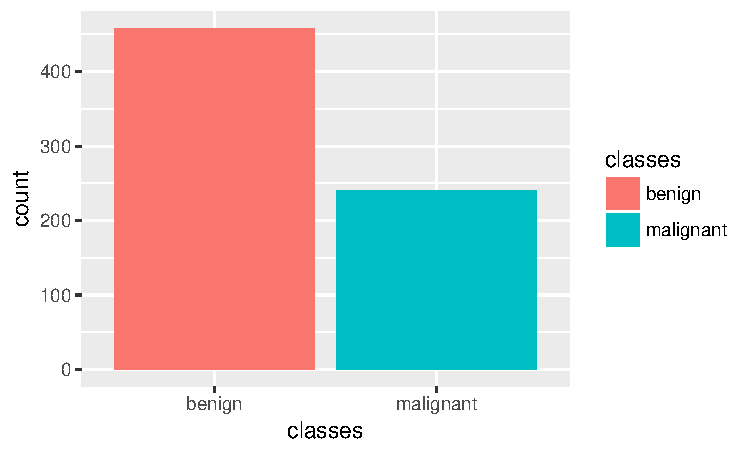
\includegraphics[width=0.9\textwidth]{webinar_code_files/figure-latex/response_classification-1.pdf}
		
		\column{0.5\textwidth}
		\centering
		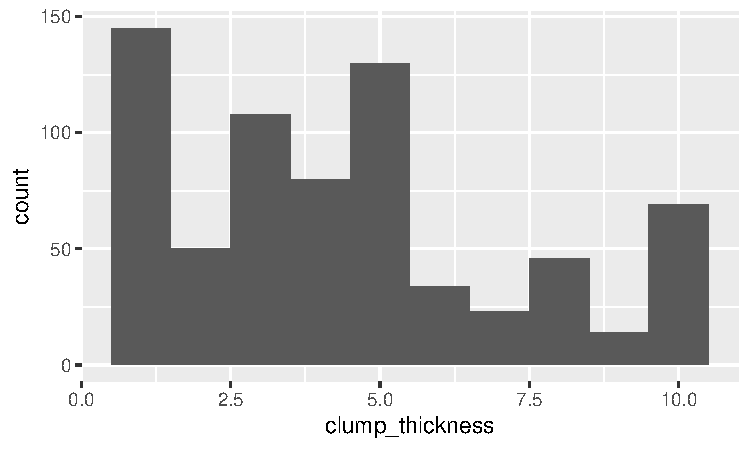
\includegraphics[width=0.9\textwidth]{webinar_code_files/figure-latex/response_regression-1.pdf}
	\end{columns}
	
		\vspace{0.5cm}

	\alert{Missing data}
	\begin{itemize}
		\item Is there missing data?
		\item Can we afford to loose data points?
		\item Or do we use imputation (and introduce additional uncertainty)?
	\end{itemize}

\end{frame}

\note{
	\begin{itemize}
		\item Before begin thinking about machine learning, we should get to know our data
		\item This is crucial to understanding the data and later on the model and it's interpretations
		\item A few basic things you can do are: Look at data types (categorical vs continuous, etc.) 
		\item Check variable classes (what is good outcome to train on). 
		\item Two specific things that are important to know for ML are:
		\item 1) the distribution: are the classes balanced?
		\item If we have unbalanced data, this will effect our model later on \\
		We would have to consider over- or undersampling.
		\item the two plots show on the left: the data used to demonstrate classification, where we want to predict the classes 'benign' or 'malignant'
		\item the right plot show the example variable used to demonstrate regression: clump thickness
		\item 2) Missing data is another important aspect for modeling
		\item If we have lots of data and few missing values, we can afford to loose these data points.
		\item If we don't have that much data though, our model will probably loose significant power if we remove the samples.
		\item In that case, we would rather introduce some uncertainty by imputing missing values. 
	\end{itemize}	
}

\begin{frame}
	\frametitle{Get to know your data}
	\alert{Principal Component Analysis (PCA)}
	
	\vspace{0.5cm}

	\centering
	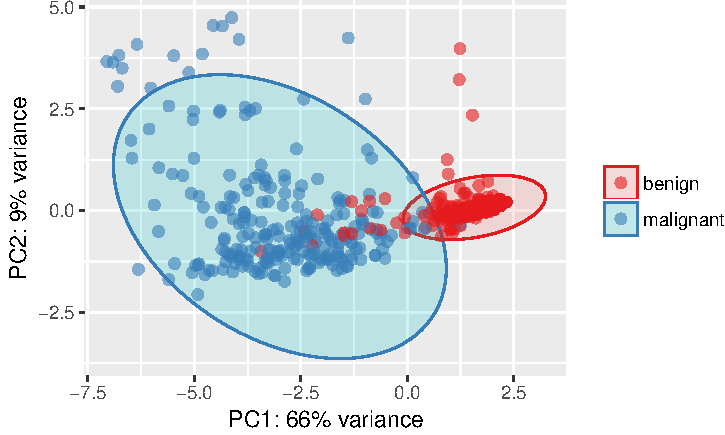
\includegraphics[width=0.9\textwidth]{webinar_code_files/figure-latex/pca-1.pdf}
\end{frame}

%\begin{frame}
%	\frametitle{Get to know your data}
%	\alert{Principal Component Analysis (PCA)}
	
%	\vspace{0.5cm}

%	\centering
%	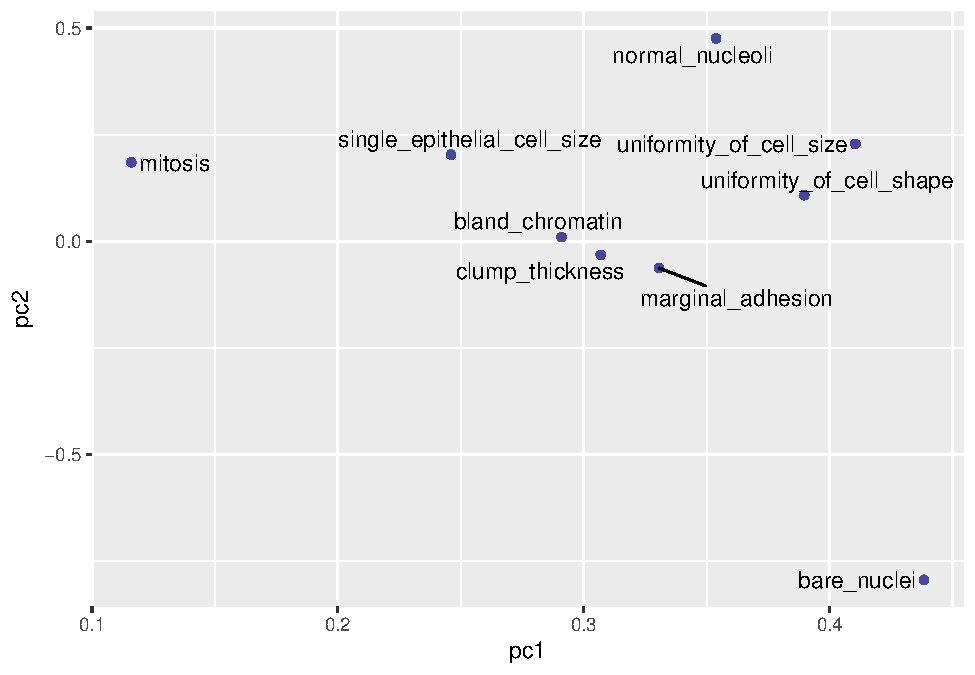
\includegraphics[width=0.8\textwidth]{webinar_code_files/figure-latex/pca_features-1.pdf}
%\end{frame}

\note{
	\begin{itemize}
		\item Most real data sets are hard to see because they have many variables and many rows
		\item visualization can help when we reduce the complexity
		\item There are many techniques for projecting the rows of a data set from a high-dimensional original space to a more visually understandable lower-dimensional space:
		\item Principal Component Analysis (PCA)
		\item Multidimensional Scaling (MDS)
		\item t-distributed Stochastic Neighbor Embedding (t-SNE)
		\item Each of these techniques has strengths and weaknesses, but the key idea they all share is to represent the rows of a data set in a meaningful low-dimensional space. 
	\end{itemize}

	\begin{itemize}
		\item To get an idea about the dimensionality and variance of the datasets, I am first looking at PCA plots
		\item Principal component analysis (PCA) is a statistical procedure that uses an orthogonal transformation ...
		\item ... to convert a set of observations into a set of values of linearly uncorrelated variables called principal components
		\item The first two principal components (PCs) show the two major trends in the data that explain the majority of variation in the data
		\item PCA can be done on any data matrix. Here I color the points by class label.
		\item From this plot, you can already see that there is a general trend in the total dataset that samples from the two classes are distinguishable: the majority of variation comes from whether a sample came from a benign or malignant mass
	\end{itemize}
}

\begin{frame}
	\frametitle{Get to know your data}
	\alert{Features}
	
	\begin{itemize}
		\item factors or numeric
		\item pre-processing
	\end{itemize}
	
	\centering
	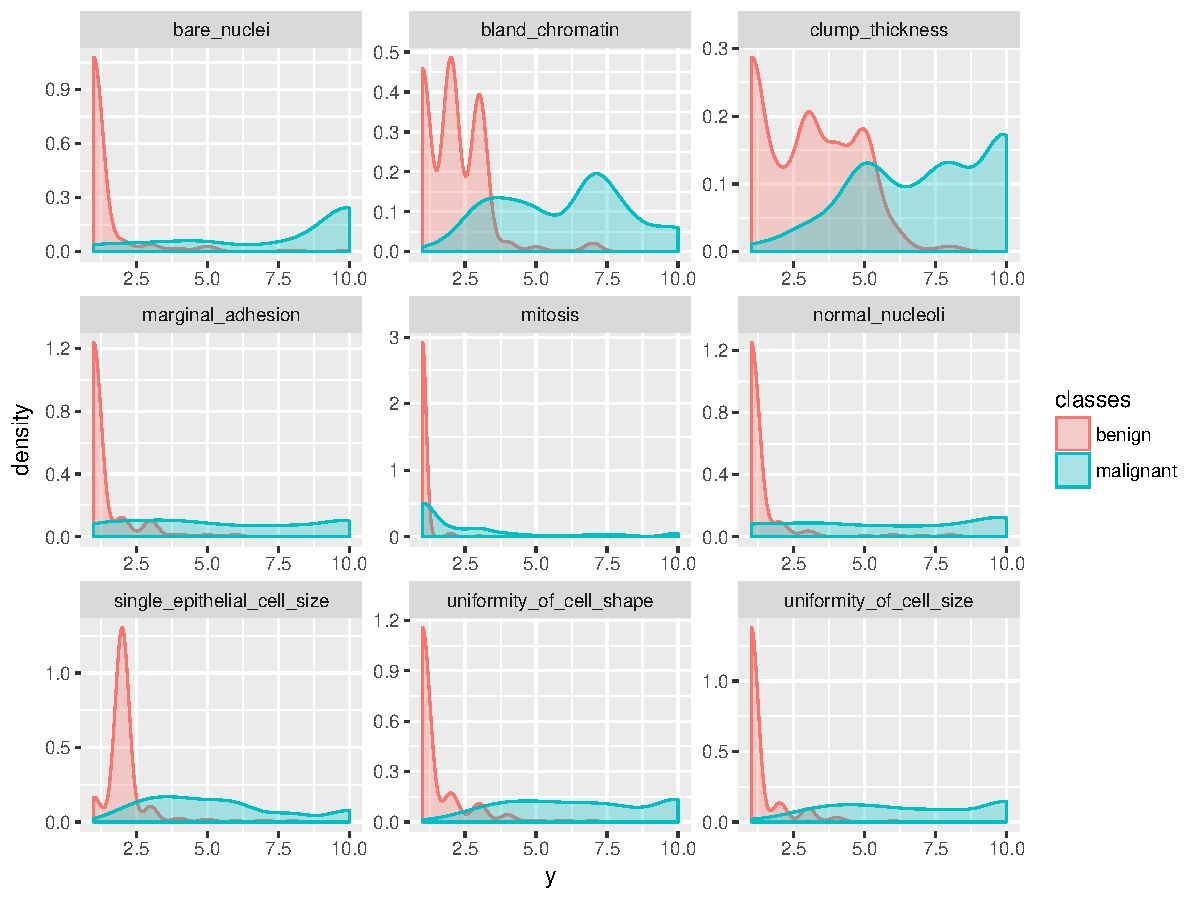
\includegraphics[width=0.7\textwidth]{webinar_code_files/figure-latex/features-1.pdf}
\end{frame}

\note{
	\begin{itemize}
		\item Next, we want to get an idea about the features.
		\item By simply plotting the distribution, we can already get a feeling of how good they are for telling apart \\ our two class labels.
		\item Here, we only have a small dataset with 9 features
		\item If you have bigger dataset, this might of course not be practical to look at individually any more.
		\item But here, we can nicely see that malignant samples seem to have a much broader range of values in all features than \\ the benign samples
		\item Based on this, we could already assume that a sample with a generally higher value in \\ most features is likely malignant
	\end{itemize}
}

\begin{frame}
	\frametitle{Get to know your data}
	\alert{Correlation}

	\centering
	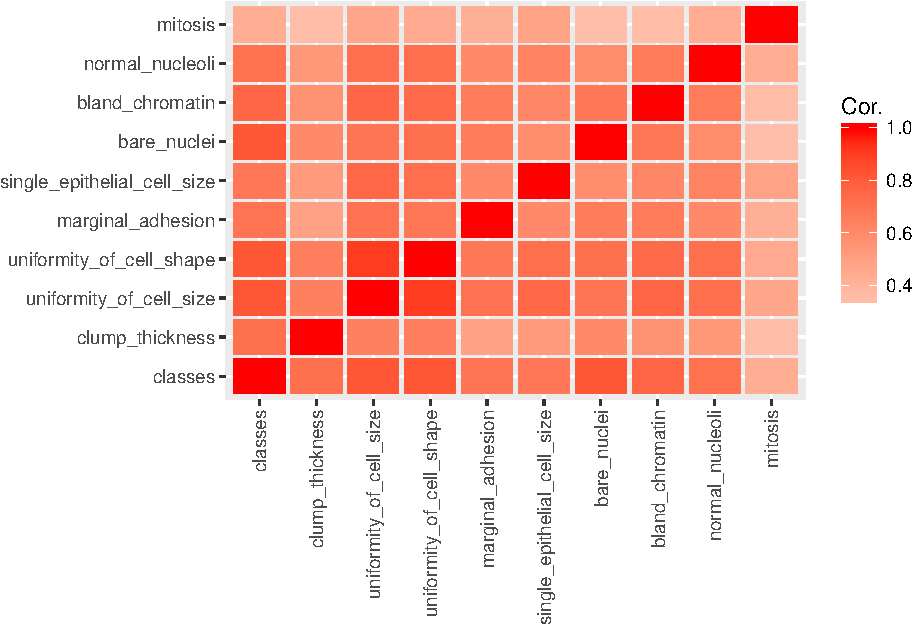
\includegraphics[width=0.9\textwidth]{webinar_code_files/figure-latex/corr_plot-1.pdf}
\end{frame}

\note{
	\begin{itemize}
		\item Correlation between features is also of interest.
		\item features with a high correlation might be regulated by common factors
		\item on the other hand, highly correlated features will also give redundant information and we might want to consider \\ either leaving only one of these features or combining them into a new engineered feature.
		\item features that are highly correlated with the classes are also probably features of high importance for the \\ prediction model later on
		\item here, I show a correlation heatmap of Pearson correlation coefficients 
		\item we can directly see that uniformity of cell shape and cell size are very highly correlated
		\item and mitosis is the one feature with comparably low correlation - also with the classes, so it likely \\ will not contribute much in terms of predictive power
	\end{itemize}
}

%\begin{frame}
%	\frametitle{Get to know your data}
%	\alert{Correlation graphs}
%
%	\begin{center}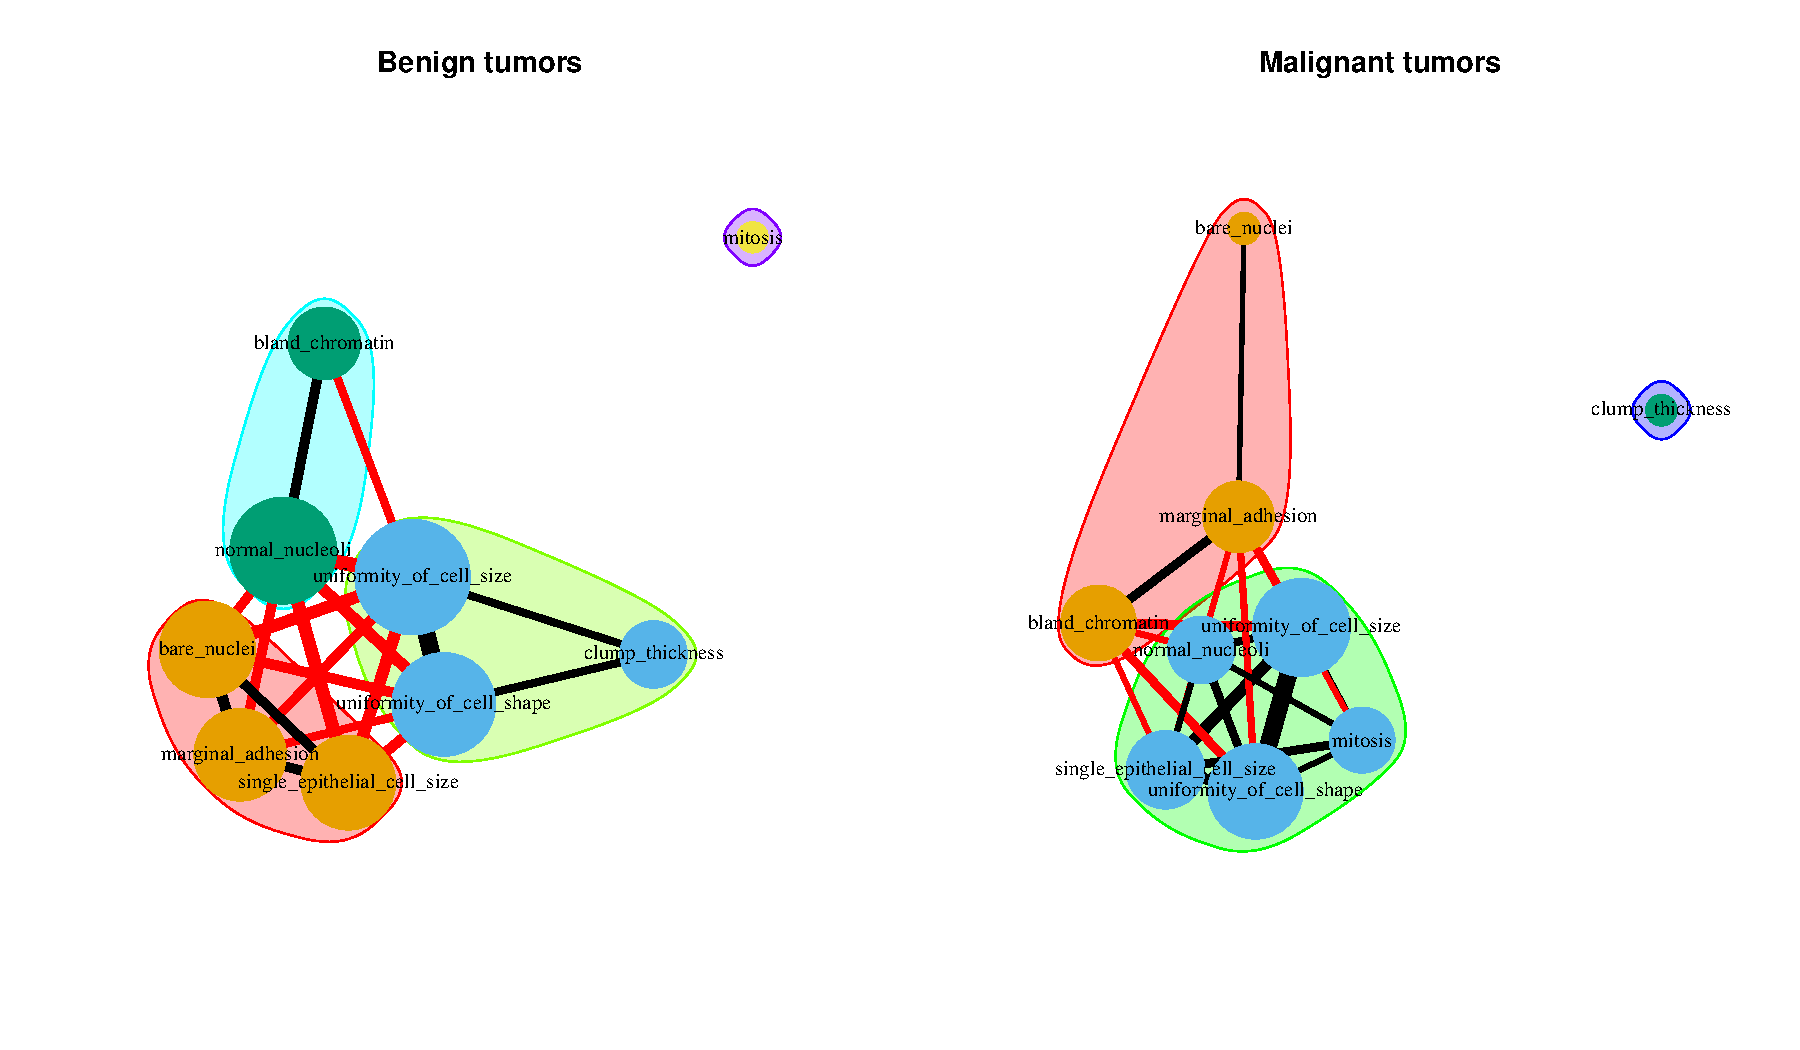
\includegraphics[width=1\textwidth]{webinar_code_files/figure-latex/cor_graph-1} \end{center}
%\end{frame}

%\note{
%	\begin{itemize}
%		\item A correlation graph is a two-dimensional representation of the relationships (correlation) in a data set
%		\item Pearson correlation coefficient between features
%		\item node size: sum of correlation coefficients
%		\item edge width: correlation coefficient
%	\end{itemize}
%}


\begin{frame}
	\frametitle{Training, validation and test data}
	
	Splitting the data into training and test sets - \\
	ideally \alert{stratified} by response class.
	
	\vspace{0.5cm}

	\alert{Density distribution}
	\begin{center}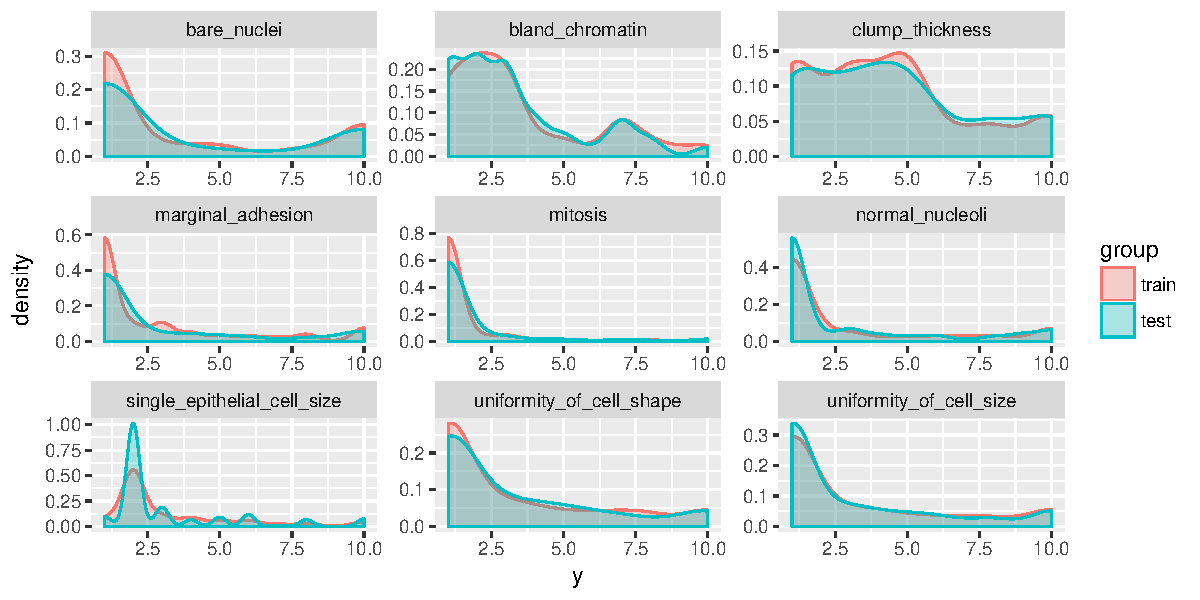
\includegraphics[width=1\textwidth]{webinar_code_files/figure-latex/distribution-1} \end{center}
\end{frame}

\note{
	\begin{itemize}
		\item We now want to split the data randomly into training and test sets
		\item the density distribution should be similar in training and test data!
	\end{itemize}
}

\begin{frame}
	\frametitle{Model examples}
	
	\begin{columns}
		
		\column{0.6\textwidth}
		
		\alert{Regression with Linear Models}
		\begin{itemize}
			\item e.g. Generalized Linear Models
			\item with \textsl{caret}
		\end{itemize}
		
		\vspace{0.5cm}
		
		\alert{Tree-based classification}
		\begin{itemize}
			\item Random Forest or Gradient boosting trees
			\item  with \textsl{caret}
		\end{itemize}
		
		\vspace{0.5cm}
		
		\alert{Hyper-parameter tuning}
		\begin{itemize}
			\item Grid Search
			\item  with \textsl{h2o}
		\end{itemize}
	
		\column{0.4\textwidth}
		
		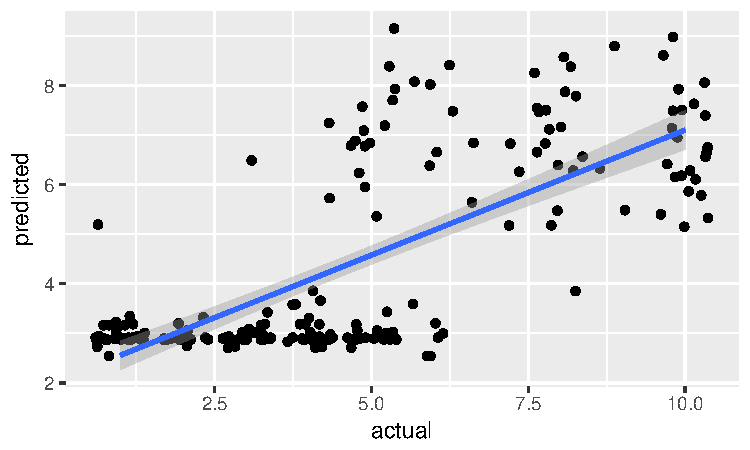
\includegraphics[width=0.9\textwidth]{webinar_code_files/figure-latex/regression_result-1.pdf}
		
		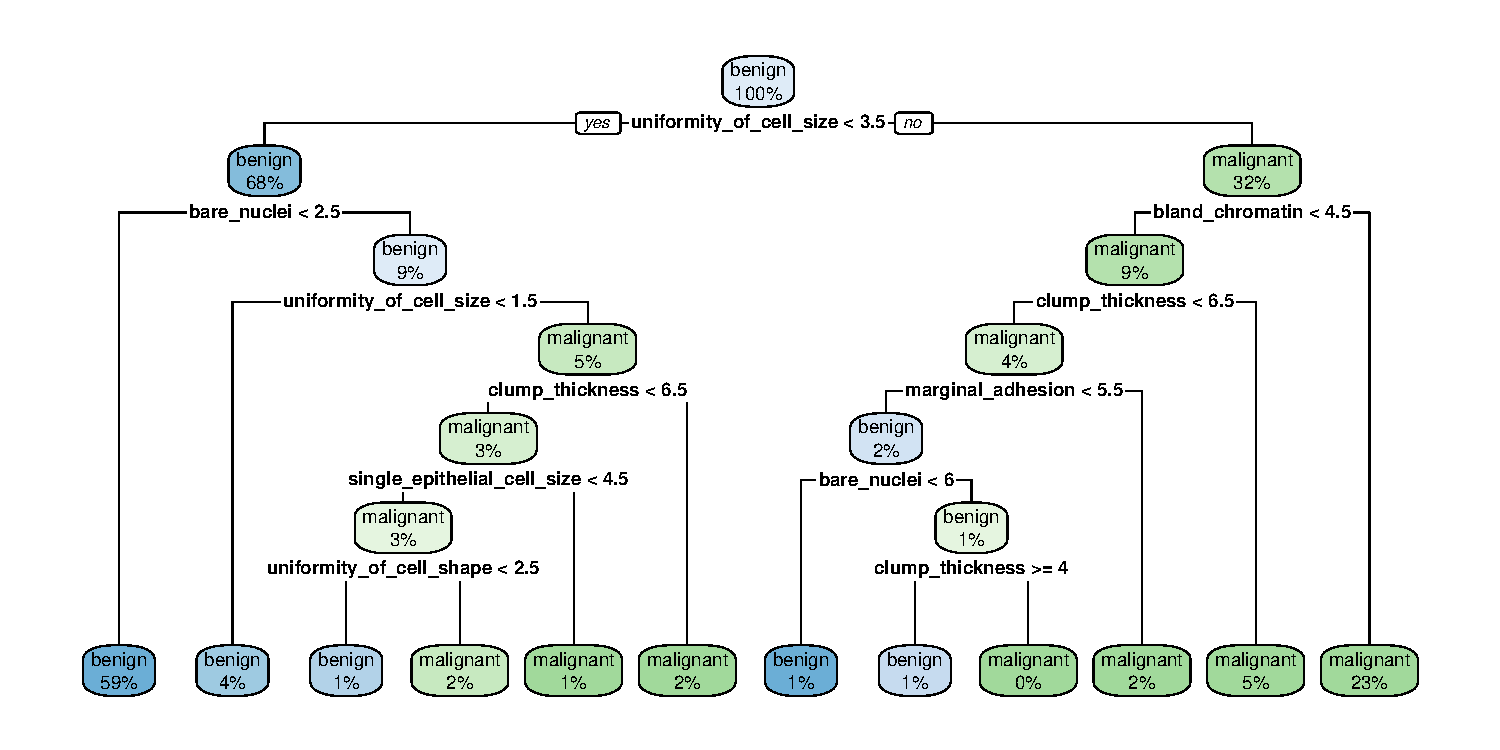
\includegraphics[width=1\textwidth]{webinar_code_files/figure-latex/decision_tree-1}
		
		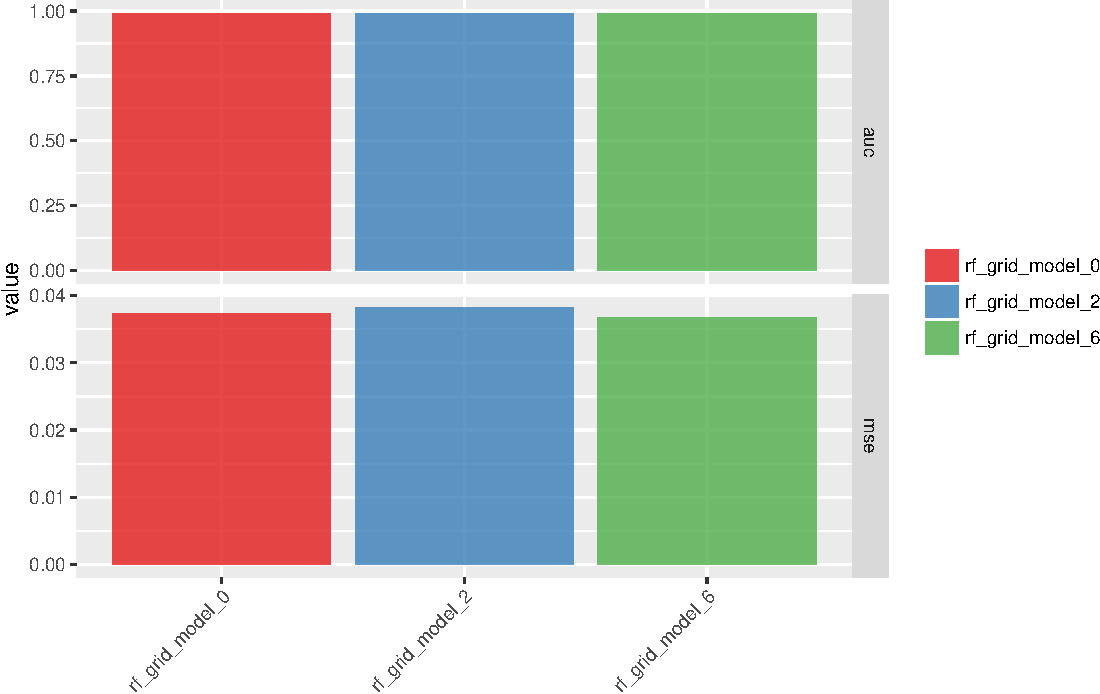
\includegraphics[width=0.9\textwidth]{webinar_code_files/figure-latex/auc_mse-1.pdf}
	\end{columns}
	
	
\end{frame}

\note{
	\begin{itemize}
		\item Now we can go ahead with actual modeling:
		\item There are over 250 ML algorithms implemented in caret alone. 
		\item But I am going to focus on two of the most widely used: GLM and RF
	\end{itemize}
	
	\begin{itemize}
		\item traditional linear models tend to create linear, monotonic, and continuous functions 
		\item Even though they're not always the most accurate predictors, the simplicity of linear models makes the results they generate easy to interpret.
		\item Random Forests are decision tree based algorithms and I will explain them in more detail in a minute
	\end{itemize}

	\begin{itemize}
		\item Of course, you need quite a bit of experience and intuition to hit on a good combination of parameters for modeling.
		\item That's why it usually makes sense to do a grid search for hyper-parameter tuning. 
		\item It allows us to test different combinations of hyper-parameters and find one with improved accuracy.
	\end{itemize}
}

\begin{frame}
	\frametitle{Classification with tree-based models}
	\alert{Decision trees} 
		
	\begin{center}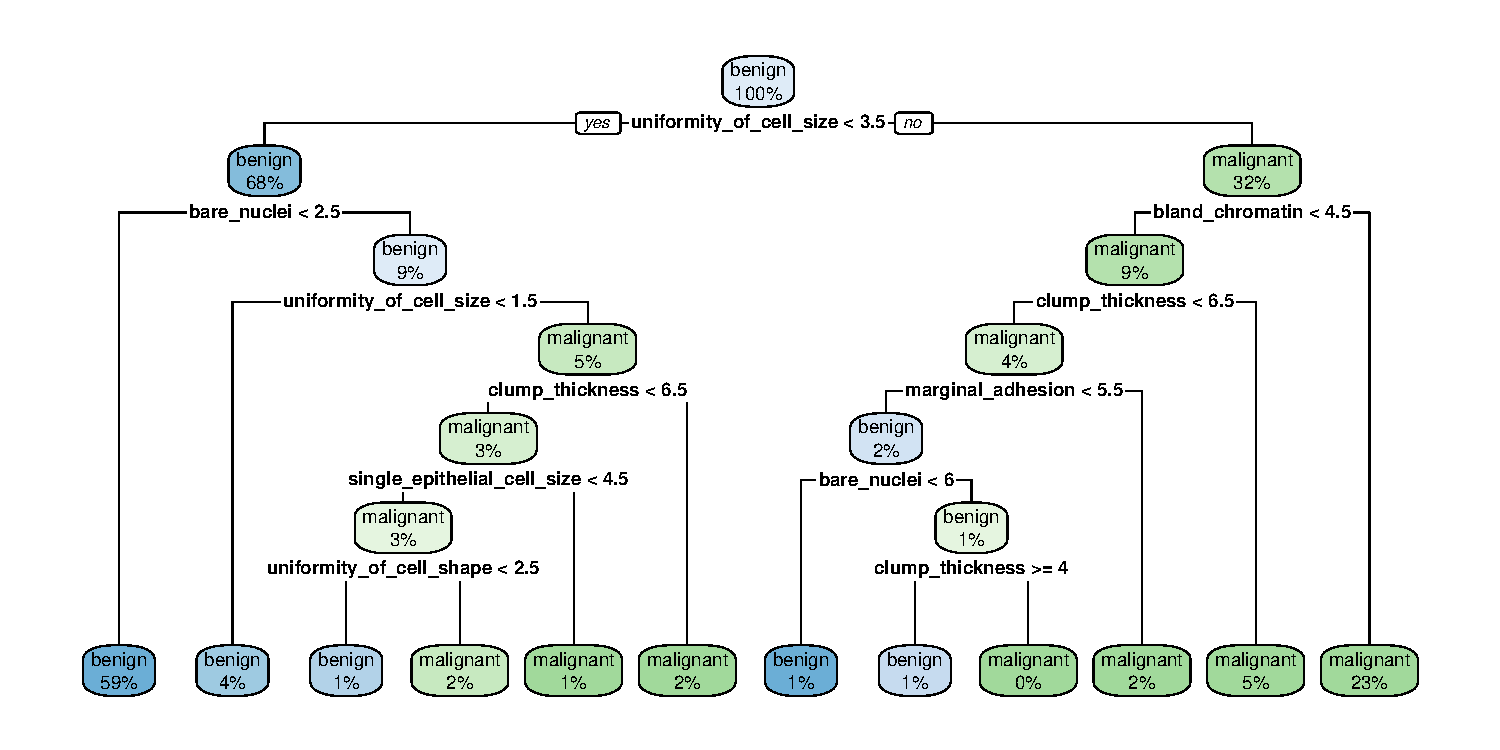
\includegraphics[width=1\textwidth]{webinar_code_files/figure-latex/decision_tree-1} \end{center}

\end{frame}

\note{
	\begin{itemize}
		\item Decision trees are the basis for Random forest and boosting trees
		\item One decision tree is built the following way:
		\item We start with a group of samples
		\item for each sample, we assign a class: e.g. it being from benign or malignant
		\item for each sample, we also have a number of features
		\item a decision trees then separates the data at several nodes to end up with classifications at the final leaves
		\item this way, the model learns a conditional structure of discriminative features
	\end{itemize}

	\begin{itemize}
		\item Random Forests produces multiple decision trees
		\item with some level of randomness
		\item Every node in the decision trees is a condition on a single feature, designed to split the dataset into two so that similar response values end up in the same set
		\item each tree is evaluated regarding how well it classified the samples (using e.g. cross-validation)
		\item an ensemble of all trees is then used for prediction
		\item this affords RF better generalization abilities than individual trees
		\item Individual trees are interpretable
		\item but with more trees and more features the final models become vastly more complex
		\item So, while theoretically we would be able to understand models based on decision trees, in reality, we usually can not
	\end{itemize}
}

\begin{frame}
	\frametitle{Feature importance}
	
	\begin{center}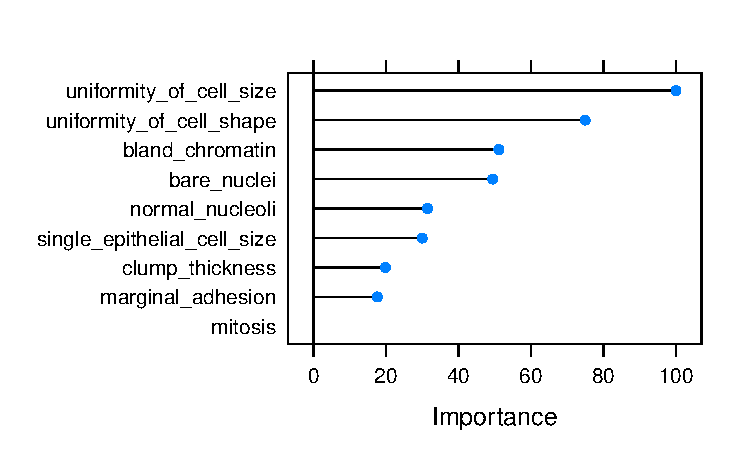
\includegraphics[width=0.8\textwidth]{webinar_code_files/figure-latex/importance_rf-1.pdf} \end{center}
\end{frame}

\note{
	\begin{itemize}
		\item Not all of the features will be equally important to the model. 
		\item A benefit of using ensembles of decision tree methods is that they can automatically provide estimates of feature importance from a trained predictive model.
		\item Generally, importance provides a score that indicates how useful or valuable each feature was \\�in the construction of the decision trees within the model. 
		\item The more an attribute is used to make key decisions with decision trees, the higher its relative importance.
		\item Importance is calculated for a single decision tree by how much each attribute split improves the performance \\ measure, weighted by the number of observations the node is responsible for.
		\item The feature importances are then averaged across all of the the decision trees within the model.
		%\item when training a tree, it can be computed how much each feature decreases the weighted impurity in a tree. For a forest, the impurity decrease from each feature can be averaged and the features are ranked according to this measure.
		\item 'information gain' is the measure that tells us how good a tree model is
		\item the measure based on which the (locally) optimal condition is chosen is called impurity. For classification, \\ it is typically either Gini impurity or information gain/entropy and for regression trees it is variance
		\item If you think back to the correlation heatmap we generated earlier, we can see that the features with the highest correlation with the output classes also have the highest importance weights!
	\end{itemize}
}

%%%%%%%%%%%%%%%%%%%%%
%	SECTION
%	Evaluating model performance
%%%%%%%%%%%%%%%%%%%%%

\section{Evaluating model performance}

\note{
	\begin{itemize}
		\item Because we usually build models that are too complex to really understand, we need other ways of assessing the trustworthiness of our models
	\end{itemize}
}

\begin{frame}[plain, c]
	\begin{center}
		\usebeamerfont*{frametitle} \usebeamercolor[fg]{frametitle} {\Huge \textbf{Never use the same data}}
		
		\vspace{0.2cm}
		
		\usebeamerfont*{frametitle} \usebeamercolor[fg]{frametitle} {\Huge \textbf{for evaluation that you used}}
		
		\vspace{0.2cm}
		
		\usebeamerfont*{frametitle} \usebeamercolor[fg]{frametitle} {\Huge \textbf{for training!}}
	\end{center}
\end{frame}

\note{
	\begin{itemize}
		\item This is the Golden Rule of ML: always test model performance on independent data
		\item otherwise you will get overly optimistic performance measures
		\item The ultimate performance test for our model will always be it's prediction accuracy on a test set it hasn't seen before.
	\end{itemize}
}

\begin{frame}
	\frametitle{Predictions on test data}
	\alert{Generalized Linear Regression (GLM)} \\ response variable: clump thickness
	
	\begin{itemize}
		\item RMSE: 1.97
		\item R\textsuperscript{2}: 0.50
	\end{itemize}
	
	\vspace{0.2cm}
	
	\centering
	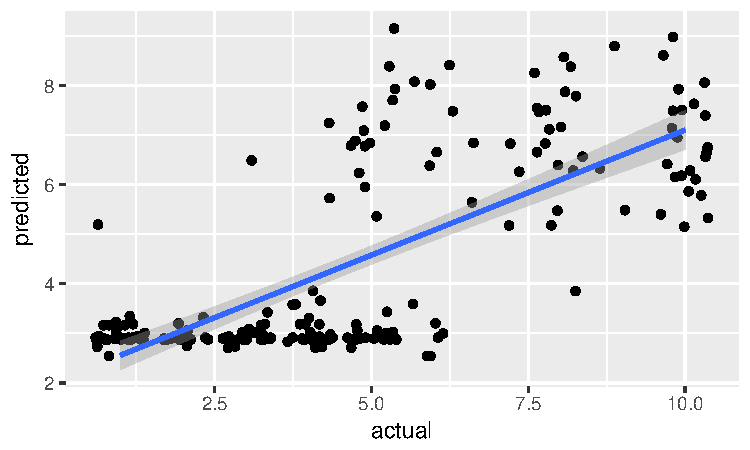
\includegraphics[width=0.5\textwidth]{webinar_code_files/figure-latex/regression_result-1.pdf}
	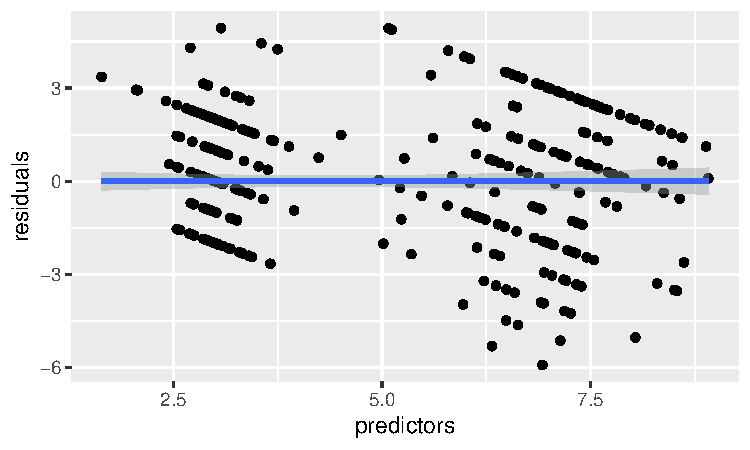
\includegraphics[width=0.5\textwidth]{webinar_code_files/figure-latex/residuals-1.pdf}
\end{frame}

\note{
	\begin{itemize}
		\item Here, you can see the results from predicting clump thickness with a GLM model
		\item To assess the accuracy, the model gives us the following output values: RMSE = root of the mean squared error and R-squared
		\item In regression analysis, the term mean squared error refers to the unbiased estimate of error variance:
		\item the residual sum of squares divided by the number of degrees of freedom
		\item in regression the predictor variable is a real number, therefore to measure the quality of the predicted value from some algorithm you need to find some sort of difference between them. You do this by calculating the square of the error, take the mean across all test objects and take square root
		\item A small RMSE means good prediction accuracy.
		\item RMSE is strongly influenced by outliers!
	\end{itemize}
	
	\begin{itemize}
		\item R-squared is the ratio of explained variance to the total variance.
		\item it is a measure of how much of the variance in y is explained by the model. If R2 is close to one, then the model's predictions are close to the true outcome
	\end{itemize}
	
	\begin{itemize}
		\item The plot on the left shows actual clump thickness (x-axis) vs predicted clump thickness from our model (y-axis)
		\item the differences between actual and predicted values are the residulas
		\item the plot on the right shows predicted values (x-axis) vs residuals (y-axis)
		\item Generally, the residuals of a well-fit model should be randomly distributed because good models will account for most phenomena in a data set, except for random error.
		\item We can conclude here, that our model was not very good at predicting clump thickness!
	\end{itemize}
}

\begin{frame}
	\frametitle{Predictions on test data}
	\alert{Classification with Random Forests}
	
	\begin{columns}
	\column{0.5\textwidth}
	
	\centering
	%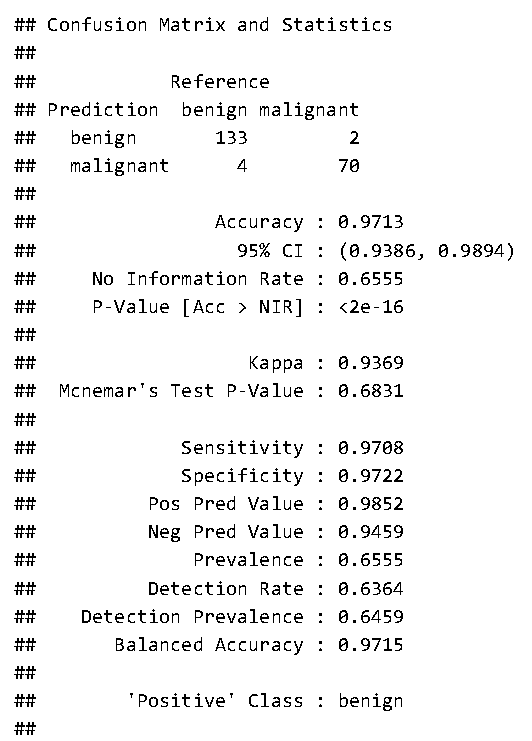
\includegraphics[width=0.9\textwidth]{images/results_matrix.pdf}

\begin{table}[]
	\centering
	\small
	\begin{tabular}{@{}rrr@{}}
		 & \textit{Reference} & \\
		 \textit{Prediction} & benign & malignant \\
		 benign & 133 & 2 \\
		 malignant & 4 & 70 \\
	\end{tabular}
\end{table}

\begin{itemize}
	\item Recall/ Sensitivity: 0.97
	\item Specificity: 0.97
	\item Accuracy: 0.97
	\item Balanced Accuracy: 0.97
\end {itemize}

	
	\column{0.5\textwidth}
	\centering	
	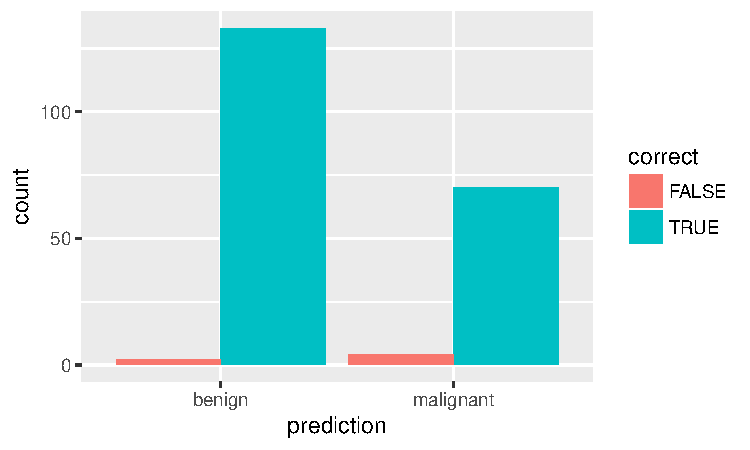
\includegraphics[width=1\textwidth]{webinar_code_files/figure-latex/results_bar_rf-1.pdf}
	
	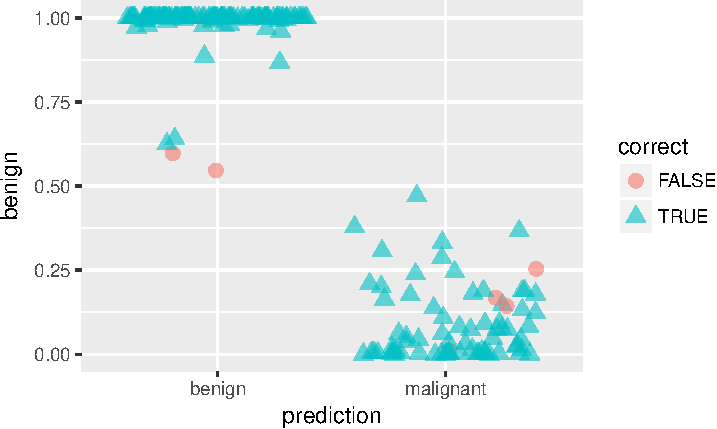
\includegraphics[width=1\textwidth]{webinar_code_files/figure-latex/results_jitter_rf-1.pdf} 
\end{columns}
\end{frame}

\note{
	\begin{itemize}
		\item Now we come to the classification models, here a example for predicting the class labels benign and malignant with Random Forests
		\item When comparing true vs predicted class labels, we can generate a confusion matrix
		\item We can also ask for a number of different measures about model performance:
		\item recall == sensitivity == True Positive Rate: proportion of positives that are correctly identified (e.g., the percentage of sick people who are correctly identified as having the condition).
		\item Specificity == True Negative Rate: proportion of negatives that are correctly identified (e.g., the percentage of healthy people who are correctly identified as not having the condition)
		\item Accuracy: is the weighted arithmetic mean of Precision and Recall
		%\item the p-value is calculated with a one-sided test to see if the accuracy is better than the "no information rate"
		%\item No Information Rate: the proportion of classes that you would guess right if you randomly allocated them
		%\item Kappa: can have values between -1 and 1. 1 or -1 show complete agreement, zero shows complete disagreement
		%\item McNemar's test: statistical test applied to 2 x 2 contingency tables to determine whether the row and column marginal frequencies are equal
		%\item positive and negative predictive values: proportions of true positive and true negative results, depend on prevalence (how often each class label occurred)
		%\item Inverse Precision and Recall: Precision and Recall where positive and negative labels are exchanged
		%\item detection rate == sensitivity
	\end{itemize}

	\begin{itemize}
		\item accuracy can be a misleading performance measure. Specifically, it may falsely suggest above-chance generalizability:
		\item in binary classification, an unbalanced dataset may result in a classifier that is biased towards the more frequent class
		\item Balanced accuracy:  average accuracy obtained on either class. Based on a confusion matrix
	\end{itemize}

	\begin{itemize}
		\item On the right, you can see the corresponding plots
		\item above: how many predictions were correct
		\item below: what prediction probabilities did our samples have if they were correctly or wrongly classified
		\item Sometimes we can already see from this whether the default threshold of 0.5 makes sense
		\item but more on prediction thresholds later
	\end{itemize}	
}

\begin{frame}
	\frametitle{Area Under the Curve (AUC)}
	
	\centering
	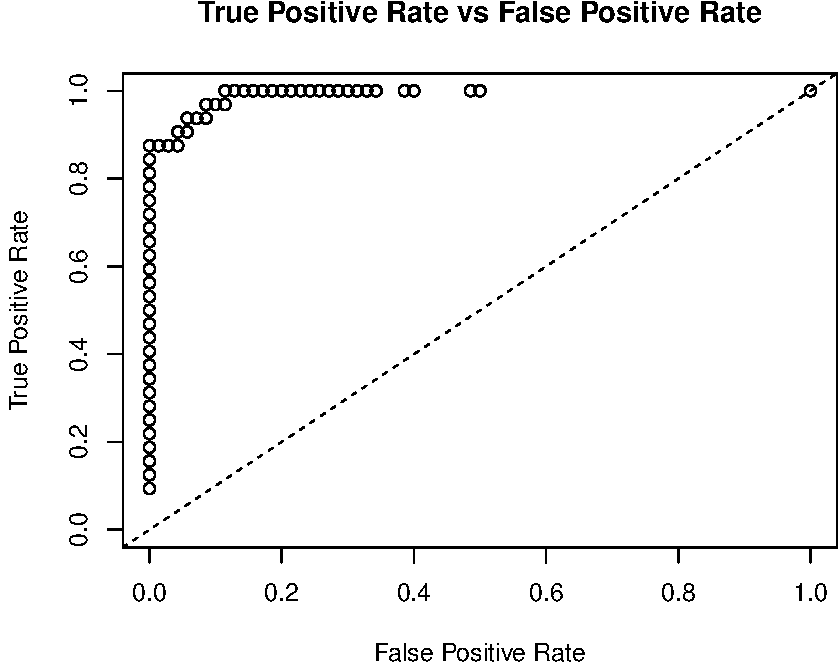
\includegraphics[width=0.8\textwidth]{webinar_code_files/figure-latex/auc_curve-1.pdf} 
\end{frame}

\note{
	\begin{itemize}
		\item AUC usually refers to area under ROC curve (mathematically known as definite integral): Receiver Operating Characteristic
		\item metric for binary classification
		\item Accuracy deals with ones and zeros, meaning you either got the class label right or you didn?t. But many classifiers are able to quantify their uncertainty about the answer by outputting a probability value.
		\item From a random classifier you can expect as many true positives as false positives. That?s the dashed line on the plot.
		\item A score for a perfect classifier would be 1
	\end{itemize}
}

\begin{frame}
	\frametitle{Hyper-parameter tuning with grid search}
	
	\begin{itemize}
		\item h2o.grid()
		\item Random Grid Search (RGS) or Cartesian Grid
	\end{itemize}

	\vspace{0.3cm}
	\alert{Define a set of hyper-parameters:}
	\begin{itemize}
		\item number of trees
		\item maximum tree depth
		\item fewest allowed (weighted) observations in a leaf
		\item etc.
	\end{itemize}

	\vspace{0.3cm}
	
	\alert{Choose best model from grid:}
	\begin{itemize}
		\item h2o.getGrid()
		\item AUC, error, accuracy, etc.
	\end{itemize}

\end{frame}

\note{
	\begin{itemize}
		\item When we build a models, we can define a number of parameters
		\item to get the best possible model, we should test different parameter combinations
		\item this, we can do with a grid search
		\item We could test all possible combinations of parameters with Cartesian Grid or exhaustive search, but Random GS \\ is much faster when we have a large number of possible combinations and usually finds sufficiently accurate models.
		\item We can use the h2o.grid() function to perform a Random Grid Search (RGS). 
		\item For RGS, we first define a set of hyper-parameters and search criteria to fine-tune our models. \\ Because there are many hyper-parameters, each with a range of possible values, we want to find an (ideally) optimal combination to maximize our model's accuracy. 
		\item We can also specify how long we want to run the grid search for.
		\item We now want to extract the best model from the grid model list. What makes a model *the best* depends \\�on the question you want to address with it: in some cases, the model with highest AUC is the most suitable, \\ or the one with the lowest mean squared error, etc. 
		\item We first use the `h2o.getGrid()` function to sort all models by the quality metric we choose \\ (depending on the metric, you want it ordered by descending or ascending values). \\�We can then get the model that's the first in the list to work with further.
	\end{itemize}
}

\begin{frame}
	\frametitle{AUC and mean squared error (MSE)}
	
	\begin{center}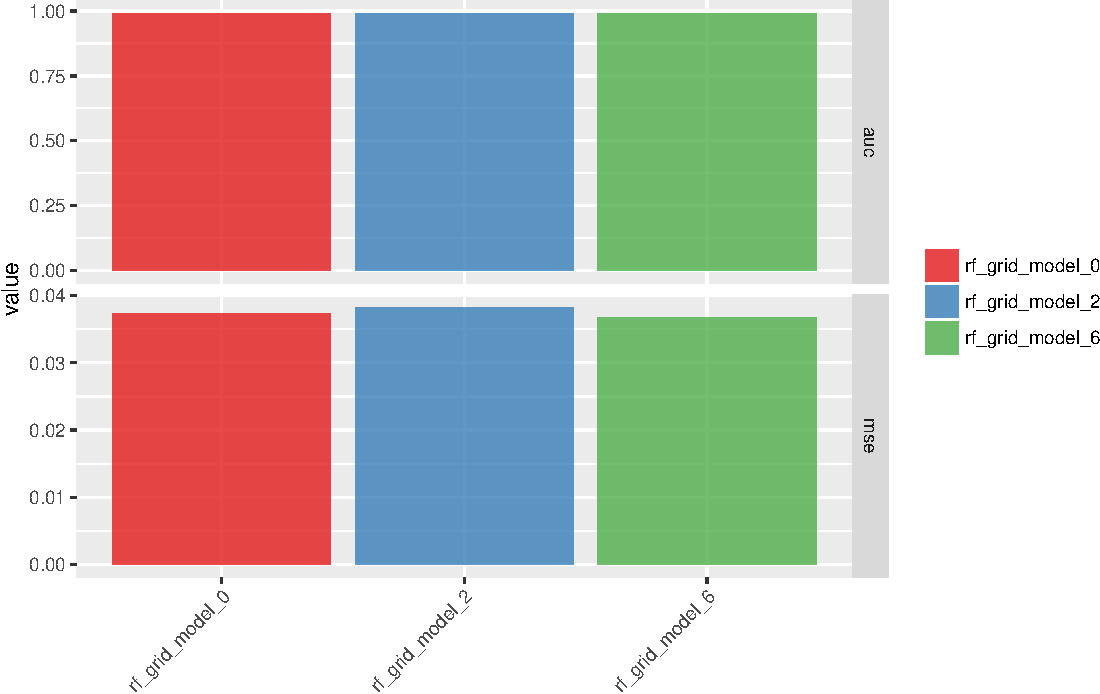
\includegraphics[width=1\textwidth]{webinar_code_files/figure-latex/auc_mse-1.pdf} \end{center}
\end{frame}

\note{
	\begin{itemize}
		\item The MSE as described for regression is a measure of the quality of an estimator. it is always non-negative, and values closer to zero are better.
	

	\end{itemize}
	%In statistics, the mean squared error (MSE) or mean squared deviation (MSD) of an estimator (of a procedure for estimating an unobserved quantity) measures the average of the squares of the errors or deviations?that is, the difference between the estimator and what is estimated. MSE is a risk function, corresponding to the expected value of the squared error loss or quadratic loss. The difference occurs because of randomness or because the estimator doesn't account for information that could produce a more accurate estimate.[1]
	
		%The MSE is the second moment (about the origin) of the error, and thus incorporates both the variance of the estimator and its bias. For an unbiased estimator, the MSE is the variance of the estimator. Like the variance, MSE has the same units of measurement as the square of the quantity being estimated. In an analogy to standard deviation, taking the square root of MSE yields the root-mean-square error or root-mean-square deviation (RMSE or RMSD), which has the same units as the quantity being estimated; for an unbiased estimator, the RMSE is the square root of the variance, known as the standard deviation.
	
	%The MSE assesses the quality of an estimator (i.e., a mathematical function mapping a sample of data to a parameter of the population from which the data is sampled) or a predictor (i.e., a function mapping arbitrary inputs to a sample of values of some random variable). Definition of an MSE differs according to whether one is describing an estimator or a predictor.
}

\begin{frame}
	\frametitle{Predictions on test data}
	
	\alert{Choosing a prediction threshold}
	
	\vspace{0.5cm}
	\centering
	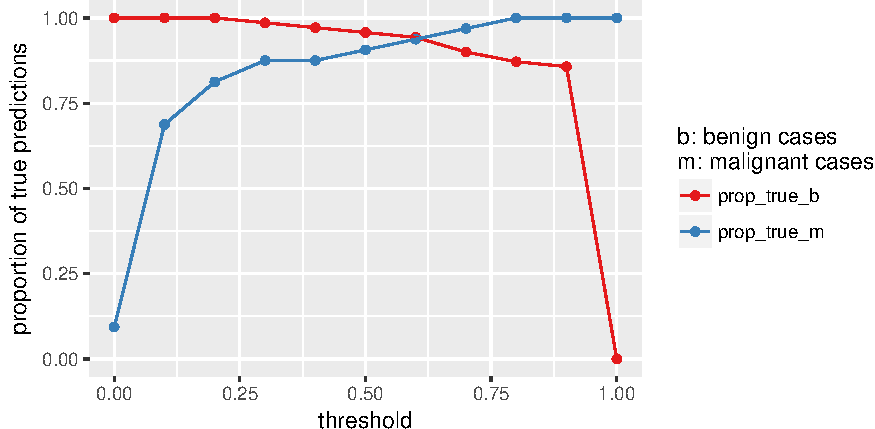
\includegraphics[width=1\textwidth]{webinar_code_files/figure-latex/prop_table-1.pdf} 
\end{frame}

\note{
	\begin{itemize}
		\item The default prediction threshold is 0.5
		\item meaning that every sample where the model give a higher prediction probability than 0.5 for benign, \\ will get predicted as benign and vice versa for malignant
		\item this threshold isn't always the best, though and we should look at the proportions of true predictions \\�for varying thresholds
		\item here, we can also choose what we want to optimize for: a balanced accuracy for the two classes \\�or do we want to maximize accuracy for one class?
	\end{itemize}
}

\begin{frame}
	\frametitle{Predictions on test data}
	
	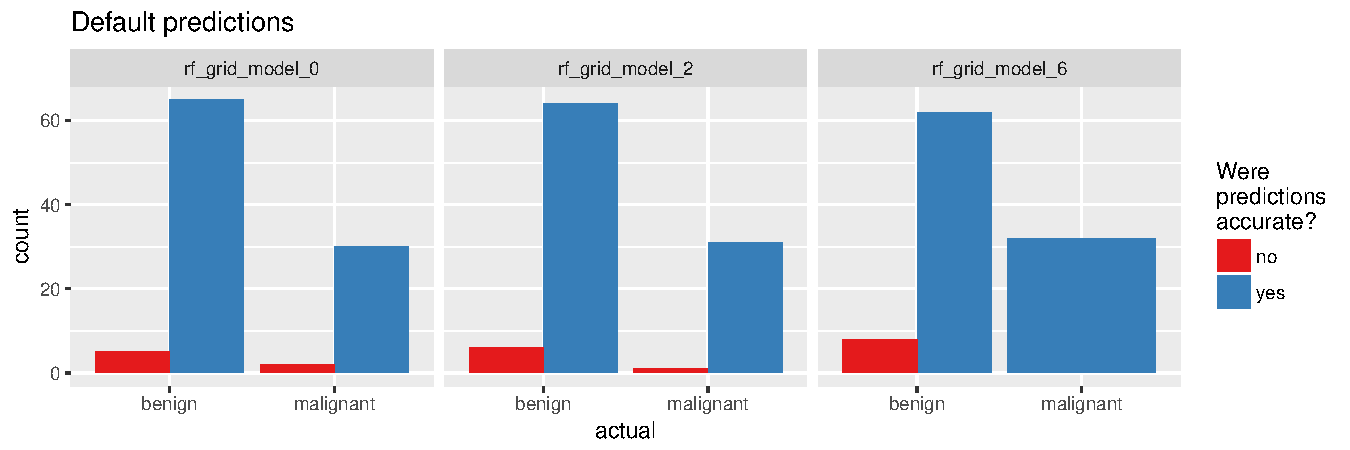
\includegraphics[width=1\textwidth]{webinar_code_files/figure-latex/final_predictions_rf-1.pdf} 

	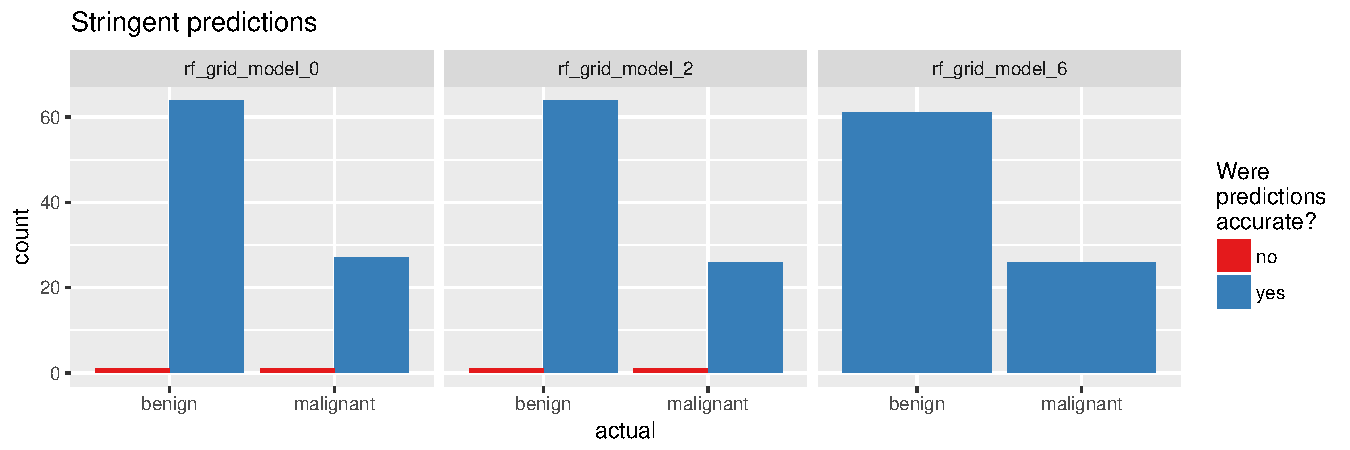
\includegraphics[width=1\textwidth]{webinar_code_files/figure-latex/final_predictions_rf-2.pdf} 
\end{frame}

\note{
	\begin{itemize}
		\item And lastly, we can compare different models' prediction accuracies
		\item and choose which one we want
		\item here you see above the default predictions with a threshold of 0.5 for three models \\
		chosen from grid search
		\item below I set a more stringent threshold of 0.8 for both classes, meaning that I loose samples between 0.2 and 0.8 and consider them uncertain
		\item now we have only correct classifications left for model 6 and could choose this for further validation we entirely new samples
	\end{itemize}
}

\begin{frame}[plain, c]
	
	\begin{center}
		\usebeamerfont*{frametitle} \usebeamercolor[fg]{frametitle} {\Huge \textbf{Take home messages:}}
	\end{center}
	
	\vspace{0.5cm}
	
	\begin{itemize}
		\item {\Large there is no 'one-size-fits-all' approach to ML}
	\end{itemize}
	
	\begin{itemize}
		\item We want to create \alert{meaningful models} that we can trust to answer our specific questions!
	\end{itemize}

	\begin{itemize}
		\item know your data well \alert{before} modeling
		\item \alert{take time to think} about pre-processing \& features
	\end{itemize}

	\begin{itemize}
		\item \alert{test} different models \& hyper-parameters
	\end{itemize}

	\begin{itemize}
		\item \alert{evaluate} model performance on independent data
		\item choose performance measure based on your \alert{specific} problem
		\item choose prediction threshold based on your \alert{specific} problem
	\end{itemize}

\end{frame}

\note{
	\begin{itemize}
		\item Just because a model performs well in the lab, doesn't mean it will also perform well in deployment
		\item the context might change: distribution, missing data, noise, class size, etc.
	\end{itemize}
}


\begin{frame}
	\frametitle{Outlook}
	
	\begin{itemize}
		\item ML could make health care more cost-effective by reducing the energy required for interpretation
	\end{itemize}

	\vspace{0.5cm}

	\begin{itemize}
		\item `Big Data' needs to be big!
		\item the more data, the more accurate the models will be
	\end{itemize}
	
	\vspace{0.5cm}
	
	\begin{itemize}	
		\item for really meaningful models, data needs to be shared
	\end{itemize}
	
	\vspace{0.5cm}
	
	\begin{itemize}
		\item issues: privacy, platform, quality standards
	\end{itemize}
\end{frame}

%%%%%%%%%%%%%%%%%%%%%

\begin{frame}[plain, c]
	
	\begin{center}
	\usebeamerfont*{frametitle} \usebeamercolor[fg]{frametitle} {\Huge \textbf{Thank you for your attention!}}
	\end{center}

	\vspace{0.5cm}

	\begin{center}
		\usebeamerfont*{frametitle} {\huge Questions?}
	\end{center}
	
	\begin{center}
	\vspace{0.5cm}
	
	Slides and code will be available on Github: \href{https://github.com/ShirinG/Webinar_ISDS}{https://github.com/ShirinG/Webinar\_ISDS} \\
	
	\vspace{0.5cm}
	
	Code will also be on my website: \\
	\href{https://shiring.github.io}{https://shiring.github.io} \\
	
	\vspace{0.5cm}
	
	You can contact me via \\
	\href{mailto:shirin.glander@wwu.de}{shirin.glander@wwu.de} \\
	
	\begin{tikzpicture}[remember picture,overlay]
	\node[xshift=-1.8cm,yshift=2cm] at (current page.south east) {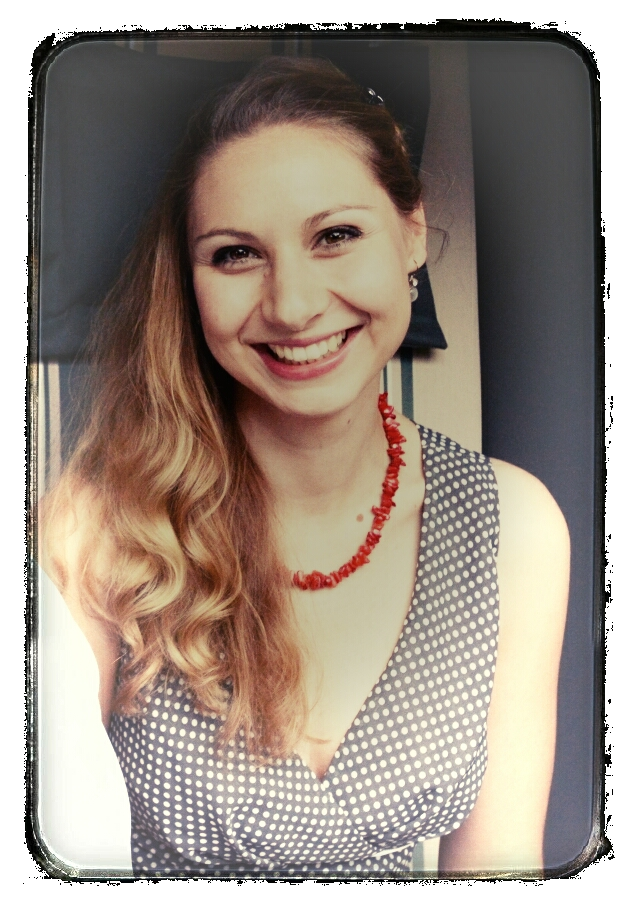
\includegraphics[width=2.5cm]{images/bild.png}};
	\end{tikzpicture}
	\end{center}
\end{frame}

\end{document}